\documentclass[11pt,letterpaper]{article}

\usepackage[utf8]{inputenc}
\usepackage[T1]{fontenc}
\usepackage{lmodern}
\usepackage[margin=1in]{geometry}
\usepackage{amsmath,amssymb}
\usepackage{booktabs}
\usepackage{longtable}
\usepackage{graphicx}
\usepackage{xcolor}
\usepackage{hyperref}
\usepackage[round,authoryear]{natbib}
\usepackage{enumitem}
\usepackage{array}
\usepackage{caption}
\usepackage{setspace}
\usepackage{tikz}
\usepackage{pgfplots}
\pgfplotsset{compat=1.18}
\usetikzlibrary{arrows.meta,positioning,calc,fit}
\usepackage{subcaption}
\usepackage[section]{placeins}

\hypersetup{hidelinks}

\title{National-Team Selection Under Pressure:\\
Graph-Scored Search and Adversarial Evaluation}
% JQAS uses blind review. Author details and acknowledgements are omitted
% from this submission copy and should be supplied separately in ScholarOne.
\author{}
\date{}

\begin{document}
\doublespacing
\maketitle

\begin{abstract}
We formulate national-team roster construction as an auditable
optimization problem that combines learned team scoring with adversarial
evaluation. A graph convolutional network, trained on historical
game-level lineups and shared-time relationships, estimates the win
probability of a candidate roster against reference opponents. Search is
performed with tournament elimination followed by batched greedy
refinement, allowing large eligible pools to be explored under explicit
roster constraints. Two domain-aware choices are central. In hockey,
positional quotas prevent degenerate optima that exploit weaknesses in
the learned scorer rather than constructing plausible teams. In
basketball, stochastic rotation scoring resolves the mismatch between a
five-player prediction model and a twelve-player roster by evaluating
empirically weighted lineup combinations for each candidate. We study
the 2025 4 Nations Face-Off and 2024 Paris men's basketball
tournaments. Constrained versions recover many core national-team
selections and avoid incoherent rosters, while unconstrained or
mismatched versions expose predictable failure modes. The results
support the method as decision support rather than an automated
selector: its value is strongest when the optimization architecture
makes assumptions explicit, preserves human-auditable constraints, and
turns model failures into diagnostic information for roster
construction. The GitHub repository and lightweight reproducibility
materials are available from the authors upon request.
\end{abstract}

\noindent\textbf{Keywords:} sports analytics; basketball; hockey;
player value; Stackelberg games; decision support

\section{Introduction}

International tournament roster construction, and adjacent high-stakes
settings such as league playoffs, are traditionally delegated to human
scouts and coaches whose judgements are opaque, inconsistent across
evaluators, and difficult to audit. We propose an alternative:
formalize roster selection as an optimization problem, where the
objective is to
\emph{maximize predicted win probability against the best response of
likely opponents}.

The approach rests on three technical components: (1) a learned
scoring function (GCN trained on game-level lineups) that predicts
win probability for any candidate roster; (2) an adversarial
evaluation framework (adversarial optimization) that tests robustness
against intelligent opponents using a leader-follower framing
\citep{conitzer2006commit}; (3) a search algorithm that navigates the
combinatorial space of valid rosters. The payoff is high: if the
components are correctly engineered, the output is reproducible,
auditable, and interpretable (via marginal player value). The risk is
high too: if any component mis-specifies the decision problem, the
output fails in catastrophic ways.

This paper presents an end-to-end prototype pipeline, identifies where
it succeeds and where it fails, and proposes architectural fixes that elevate it
from an interesting prototype to a promising decision-support
prototype. We evaluate it through case studies on 2025 4 Nations
Face-Off hockey (Canada) and 2024 Paris basketball (USA, Canada),
showing that constrained versions recover many core national-team
selections while avoiding pathological roster structures.

\section{Approach}
\label{sec:approach}

\begin{figure}[htbp]
  \centering
  \small
  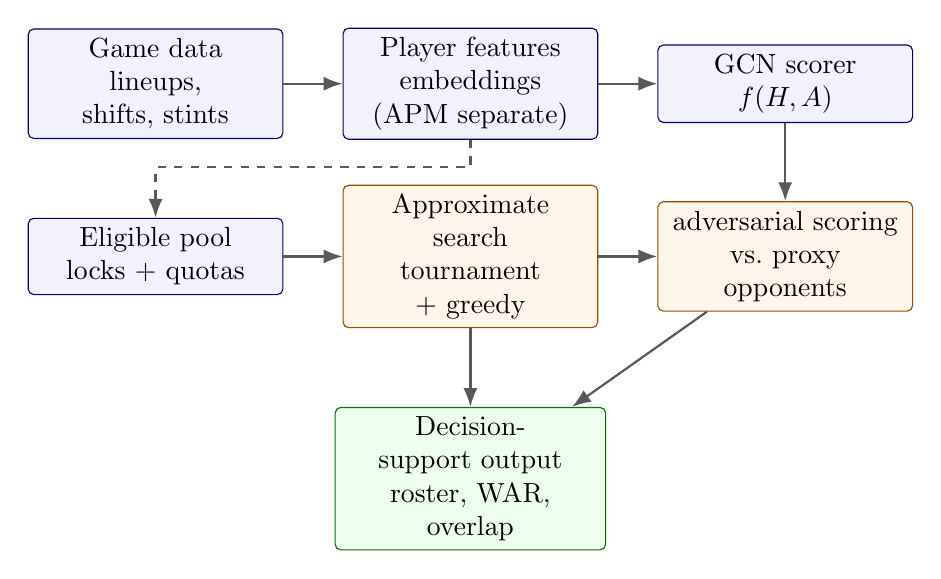
\begin{tikzpicture}[
    box/.style={
      draw=blue!45!black,
      fill=blue!5,
      rounded corners=2pt,
      align=center,
      text width=3.0cm,
      minimum height=0.9cm
    },
    evalbox/.style={
      draw=orange!60!black,
      fill=orange!8,
      rounded corners=2pt,
      align=center,
      text width=3.0cm,
      minimum height=0.9cm
    },
    outbox/.style={
      draw=green!45!black,
      fill=green!7,
      rounded corners=2pt,
      align=center,
      text width=3.2cm,
      minimum height=0.9cm
    },
    arrow/.style={-{Latex[length=2.4mm]}, thick, draw=gray!70!black},
    node distance=0.75cm and 0.75cm
  ]
    \node[box] (data) {Game data\\lineups, shifts, stints};
    \node[box, right=of data] (features) {Player features\\embeddings (APM separate)};
    \node[box, right=of features] (gcn) {GCN scorer\\$f(H,A)$};

    \node[box, below=1.0cm of data] (pool) {Eligible pool\\locks + quotas};
    \node[evalbox, right=of pool] (search) {Approximate search\\tournament + greedy};
    \node[evalbox, right=of search] (stack) {adversarial scoring\\vs.\ proxy opponents};

    \node[outbox, below=1.0cm of search] (final) {Decision-support output\\roster, WAR, overlap};

    \draw[arrow] (data) -- (features);
    \draw[arrow] (features) -- (gcn);
    \draw[arrow] (pool) -- (search);
    \draw[arrow] (gcn) -- (stack);
    \draw[arrow] (search) -- (stack);
    \draw[arrow] (stack) -- (final);
    \draw[arrow] (search) -- (final);
    \draw[arrow, dashed] (features.south) -- ++(0,-0.35) -| (pool.north);
  \end{tikzpicture}
  \caption{End-to-end prototype pipeline. Learned player features feed a
    GCN scorer, while the roster search uses locks and domain constraints
    to keep candidate teams in a plausible region of roster space.}
  \label{fig:pipeline}
\end{figure}

\subsection{Data}

\paragraph{Hockey.} NHL play-by-play, shift, and boxscore data for
seasons 2021--22 through 2025--26 were sourced from NHL public data
endpoints \citep{nhlPublicApi}. Per-game lineup stints give pairwise
on-ice time between every pair of players; an adjusted plus-minus (APM)
is fit by ridge regression on lineup indicator matrices with score
differential as the target \citep{hoerl1970ridge,macdonald2011nhl}, and
used separately for player ranking and rotation ordering. Each
player-season is encoded as a
$14$-dimensional feature vector (shot/attempt rates, xG, zone-start
percentages, TOI, height, weight, position flags). APM is intentionally
excluded from the feature vector to avoid circularity: it is validated
against public RAPM-style estimates as a standalone ranking signal, not
as an embedding component \citep{sill2010rapm,ghimire2020rapm}.

\paragraph{Basketball.} Kaggle NBA SQLite data
\citep{walshBasketball,walshNbadb}.
The initial pipeline covered only 2021--22 and 2022--23 ($\sim 2{,}400$
games); we expanded to 2019--20 through 2023--24 ($\sim 6{,}100$ games),
nearly tripling the training set and improving model stability on
held-out folds. We derive starting lineups from the first five distinct
player IDs per team in each game's period~1 of play-by-play. APM is
computed analogously to hockey and used separately for player ranking,
rotation ordering, and locked-player selection
\citep{sill2010rapm,ghimire2020rapm}; it is \emph{not} included in the
feature vector passed to the GCN, so that the RAPM correlation check
(Section~\ref{sec:rapm}) constitutes a valid
independent validation of the ranking signal rather than a circular
self-check. The initial feature vector was $13$-dimensional (FGA, FGM,
xPPP, 3pt attempts, zone dummies, position flags, height, weight, TOI);
we expanded to $23$ dimensions by replacing the coarse 5-zone shot
distribution with a finer 7-zone breakdown (restricted area, paint
non-RA, short mid-range $<$16\,ft, long mid-range 16--22\,ft, left
corner 3, right corner 3, above-the-break 3) and replacing the two
aggregate assist features with three zone-aware assist features (assist
rate, proportion of assists to 3-point shots, proportion of assists to
paint shots). The finer zone breakdown reduces the conflation of
stylistically distinct scorers: a paint-finisher and a pull-up
mid-range scorer both appeared in ``mid-range'' under the coarse scheme
despite having different spacing implications. Zone-specific assist
proportions similarly distinguish playmakers who create paint touches
from those who generate catch-and-shoot 3s, improving complementarity
inference for novel pairings.
The final basketball case studies use this $23$-dimensional feature
set.

For the reported hockey runs, player embeddings are three-year averages
over $\{y-2, y-1, y\}$. Current-year embeddings only are treated as a
future improvement rather than a reported result.

\subsection{Scoring model}

We use a Graph Convolutional Network with three design constraints that
ensure the model respects the symmetry of the problem
\citep{kipf2017gcn}:

\begin{enumerate}[leftmargin=*]
  \item \textbf{Relational convolution:} A 6-layer GCN (hidden dim 128)
    propagates player features ($\mathbf{h}_i$) along edges weighted by
    shared on-ice/on-court time. This captures indirect player
    relationships (chemistry through common teammates) rather than only
    direct co-occurrence.
  \item \textbf{Permutation-invariant aggregation:} A DeepSet layer
    independently summarizes the home and away rosters, producing
    lineup-level embeddings $\mathbf{z}_H$ and $\mathbf{z}_A$
    \citep{zaheer2017deepsets}.
  \item \textbf{Antisymmetric prediction:} The output head enforces
    $f(\mathbf{H}, \mathbf{A}) = 1 - f(\mathbf{A}, \mathbf{H})$,
    ensuring that home advantage is modeled as an additive shift rather
    than baked into the learned features.
\end{enumerate}

Training target: $y = \sigma(\Delta / 10)$ where $\Delta$ is goal/point
differential. We train an ensemble of 6 cross-validation folds using
Adamax, cosine LR schedule, MSE loss, and gradient clipping
\citep{kingma2015adam,loshchilov2017sgdr}. Predictions are averaged at
inference.

Sizes: hockey uses $n = 36$ graph nodes (18 home + 18 away), matching
the full dressed skater side. Basketball uses $n = 10$ (5-on-5 on
court) with $23$-dimensional player features, which matches the game
but not our search target of 12-player rosters, a mismatch we address
in Section~\ref{sec:arch-mismatch}.

\subsection{Adversarial Evaluation}

For a fixed candidate roster, we evaluate its predicted win probability
against $3$ reference opponents by simulating a leader-follower game
\citep{conitzer2006commit}:

\begin{itemize}[leftmargin=*]
  \item The \textbf{leader} (our candidate) picks a deployment strategy
    $\mathbf{S}$ (an $n \times n$ adjacency-style matrix) to
    \emph{maximize} $f(\mathbf{S}; \text{home}, \text{away})$.
  \item The \textbf{follower} (opponent) picks a deployment
    $\mathbf{S}'$ to \emph{minimize} the leader's payoff.
\end{itemize}

In practice, $\mathbf{S}$ parameterizes deployable co-occurrence
weights among the selected players. Player node features are fixed
during adversarial evaluation; only the interaction graph passed to the
GCN changes. Same-team blocks are constrained to be nonnegative,
cross-team blocks are constrained to be nonpositive, the diagonal is
zeroed, and a projection step fixes block-level mass and symmetrizes the
matrix so the optimizer cannot improve the score by trivially scaling
all edges.
Intuitively, same-team weights represent deployable
chemistry/co-occurrence, while cross-team weights represent adversarial
matchup pressure.

\begin{figure}[htbp]
  \centering
  \small
  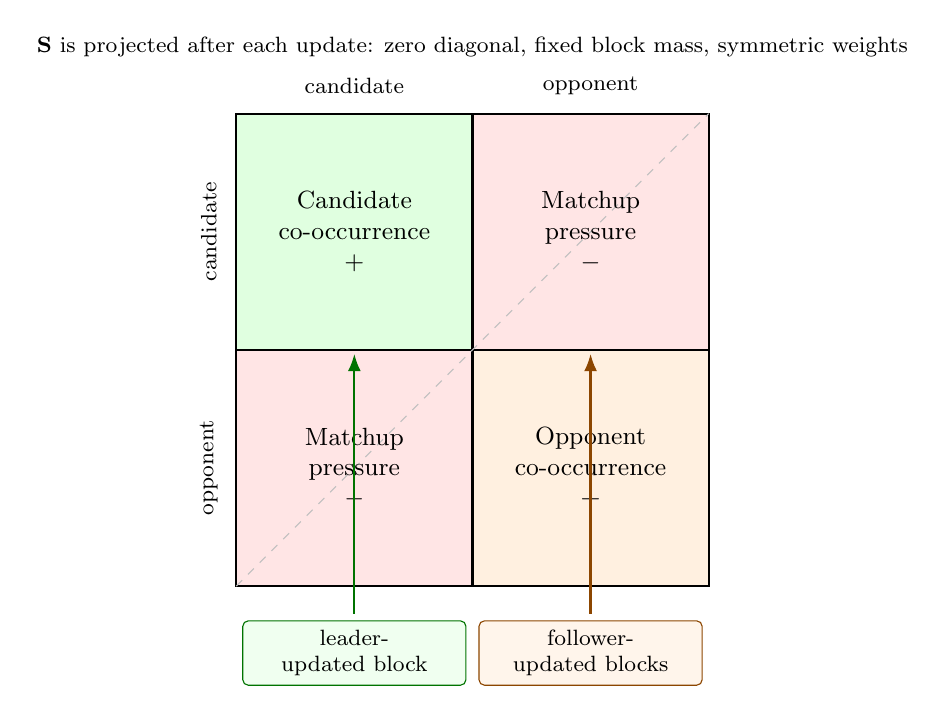
\begin{tikzpicture}[
    blocklabel/.style={align=center, font=\small},
    note/.style={align=center, font=\footnotesize, text width=2.6cm},
    axislabel/.style={font=\footnotesize}
  ]
    \fill[green!12] (0,3) rectangle (3,6);
    \fill[red!10] (3,3) rectangle (6,6);
    \fill[red!10] (0,0) rectangle (3,3);
    \fill[orange!12] (3,0) rectangle (6,3);
    \draw[thick] (0,0) rectangle (6,6);
    \draw[thick] (3,0) -- (3,6);
    \draw[thick] (0,3) -- (6,3);
    \draw[gray!50, dashed] (0,0) -- (6,6);

    \node[blocklabel] at (1.5,4.5) {Candidate\\co-occurrence\\$+$};
    \node[blocklabel] at (4.5,1.5) {Opponent\\co-occurrence\\$+$};
    \node[blocklabel] at (4.5,4.5) {Matchup\\pressure\\$-$};
    \node[blocklabel] at (1.5,1.5) {Matchup\\pressure\\$-$};

    \node[axislabel] at (1.5,6.35) {candidate};
    \node[axislabel] at (4.5,6.35) {opponent};
    \node[axislabel, rotate=90] at (-0.35,4.5) {candidate};
    \node[axislabel, rotate=90] at (-0.35,1.5) {opponent};

    \node[note, draw=green!45!black, fill=green!6, rounded corners=2pt]
      at (1.5,-0.85) {leader-updated block};
    \node[note, draw=orange!55!black, fill=orange!8, rounded corners=2pt]
      at (4.5,-0.85) {follower-updated blocks};
    \draw[-{Latex[length=2.2mm]}, draw=green!45!black, thick]
      (1.5,-0.35) -- (1.5,2.95);
    \draw[-{Latex[length=2.2mm]}, draw=orange!55!black, thick]
      (4.5,-0.35) -- (4.5,2.95);

    \node[font=\footnotesize, align=center] at (3,6.85)
      {$\mathbf{S}$ is projected after each update: zero diagonal, fixed block mass, symmetric weights};
  \end{tikzpicture}
  \caption{Schematic of the adversarial adjacency matrix. The leader
    adjusts the candidate's internal deployment graph; the follower
    adjusts opponent deployment and cross-team matchup pressure before
    the GCN scores the candidate roster.}
  \label{fig:adversarial-matrix}
\end{figure}

Both sides run $100$ gradient steps with leader-update cadence $5{:}1$
and early stopping on plateaus. The final score is
$\frac{1}{|O|}\sum_{o \in O} f(\mathbf{S}^{\star}_o, \text{opp}_o)$,
averaged across opponents $O$. For hockey, opponents are USA plus two
proxy NHL clubs (EDM and FLA), not complete international-tournament
opponent coverage. For basketball, USA evaluates against Canada,
France, and OKC, while Canada evaluates against USA, France, and OKC.

\subsection{Search}

\paragraph{Phase A Tournament.} From the full eligible pool, form
random teams of the target size (including any pre-locked stars);
evaluate each; top third of teams survive intact; in the bottom
two-thirds eliminate the lowest-usage players from each. Repeat until
roughly twice the target size remains.

\paragraph{Phase B Greedy 1-swap.} Trim to the exact target size.
Each iteration, for every non-locked slot and every bench candidate,
construct the swap-candidate lineup. Evaluate all candidates in a
single batched forward pass over \texttt{adversarial()}; pick the best
improvement. Stop on convergence or a fixed \texttt{max\_iters} cap.
This search is approximate: tournament pruning and greedy 1-swap do not
guarantee global optimality, but they make evaluation tractable under
expensive adversarial scoring.

\paragraph{Individual WAR.} For the final roster, marginal player value
is the score drop when replacing a single player with a sentinel
feature vector:
\[
  \mathrm{WAR}_i = \hat{y}(\text{full})
  - \hat{y}(\text{lineup}_{\setminus i}).
\]
Higher is better; negative values indicate the model thinks the
overall lineup is internally inconsistent.
All-positive WAR should be interpreted as a coherence diagnostic
conditional on the selected roster and opponent set, not as a
transferable estimate of player quality.

\paragraph{GroupWAR.} While individual WAR measures one player's
marginal contribution to a fixed roster, GroupWAR is the roster-level
sum of those one-player knockouts against the same opponent set. For a
selected roster $R$ with $n$ players and score $\hat{y}(R)$:
\[
  \mathrm{GroupWAR}(R) = \sum_{i \in R} \mathrm{WAR}_i(R)
  = n\cdot\hat{y}(R) - \sum_{i \in R}\hat{y}(R_{\setminus i}).
\]
A roster with high GroupWAR has no passengers: every player's removal
would meaningfully reduce the team's predicted win probability under
the same roster context and opponent set. GroupWAR is used in
Section~\ref{sec:rapm} to validate the ranking signal against public
RAPM across the full eligible pool.

\section{Results}
\label{sec:results}

Across these case studies, constrained versions recover many core
national-team selections while avoiding pathological roster structures.
Hockey dresses 18 skaters, so the 18-player dressed-roster graph better
matches the selection decision than basketball's 12-player roster /
5-player lineup mismatch.

\begin{table}[htbp]
  \centering
  \scriptsize
  \caption{Validation summary. Overlap is computed against the
    reference set named in each case study; all-positive WAR is a
    conditional coherence diagnostic, not proof of optimality.}
  \begin{tabular}{@{}l c c c p{5.0cm} c@{}}
    \toprule
    Case & Score & Ref. & Overlap & Constraint/rotation & All-pos. WAR? \\
    \midrule
    Canada hockey 2025 4 Nations & 0.4495 & 13 & 9 & loose skater-balance screen: $\geq 3$ LW, $\geq 3$ RW, 6D target; observed mix 6C/3L/3R/6D & yes \\
    Canada hockey 2024 diagnostic & 0.4428 & -- & not claimed$^\dagger$ & $\geq 3$ LW, $\geq 3$ RW, $\leq 5$ C, 6D target; observed mix 5C/4L/3R/6D & yes \\
    USA basketball 2024 & 0.7418 & 12 & 8 & stochastic 5-man rotation scoring & yes \\
    Canada basketball 2024 & 0.6587 & 12 & 9 & stochastic 5-man rotation scoring & yes \\
    \bottomrule
  \end{tabular}
  \par\smallskip
  {\scriptsize $^\dagger$ The 2024 diagnostic is a constraint-comparison study, not a roster
  recommendation; no reference overlap is claimed.}
\end{table}

\subsection{Hockey}

\subsubsection{Canada 2025}

\begin{table}[htbp]
  \centering
  \small
  \caption{Canada 2025 4 Nations Face-Off hockey case roster.
    adversarial team score $= 0.4495$; observed position mix is
    6C/3L/3R/6D under a loose skater-balance screen ($\geq 3$ LW,
    $\geq 3$ RW, 6D target). All 18 players have positive WAR.}
  \begin{tabular}{r l c c r}
    \toprule
    \# & Player & Pos & Team & WAR \\
    \midrule
    1  & Colton Parayko     & D & STL & $+0.0179$ \\
    2  & Cale Makar$^{\star}$          & D & COL & $+0.0161$ \\
    3  & Matt Duchene       & C & DAL & $+0.0150$ \\
    4  & Andrew Mangiapane  & L & EDM & $+0.0132$ \\
    5  & Sam Reinhart       & C & FLA & $+0.0130$ \\
    6  & Drew Doughty       & D & LAK & $+0.0116$ \\
    7  & Sidney Crosby$^{\star}$       & C & PIT & $+0.0105$ \\
    8  & Warren Foegele     & L & LAK & $+0.0100$ \\
    9  & Mark Stone         & R & VGK & $+0.0100$ \\
    10 & Nathan MacKinnon$^{\star}$    & C & COL & $+0.0094$ \\
    11 & Adam Henrique      & C & EDM & $+0.0085$ \\
    12 & Mario Ferraro      & D & SJS & $+0.0077$ \\
    13 & Shea Theodore$^{\star}$       & D & VGK & $+0.0061$ \\
    14 & Braeden Bowman     & R & VGK & $+0.0051$ \\
    15 & Connor McDavid$^{\star}$      & C & EDM & $+0.0050$ \\
    16 & Sean Walker        & D & CAR & $+0.0050$ \\
    17 & Lawson Crouse      & L & UTA & $+0.0022$ \\
    18 & Reilly Smith       & R & VGK & $+0.0006$ \\
    \bottomrule
  \end{tabular}
  \par \footnotesize{$^{\star}$pre-locked.}
\end{table}

The 2025 roster recovers 9 of 13 pre-identified 4 Nations Face-Off
core/reference selections
(McDavid, MacKinnon, Crosby, Makar, Theodore, Doughty, Parayko, Stone,
Reinhart) plus 9 model-selected depth contributors. This reference set
is derived from official 4 Nations roster sources
\citep{hockeyCanada4Nations,nhlFourNationsRosters}. The pipeline
correctly identifies the elite core but adds role players (Henrique,
Foegele) where team balance is marginal gain over individual talent.

\begin{table}[htbp]
  \centering
  \small
  \caption{Canada 2025 4 Nations Face-Off core/reference subset used
    for overlap accounting. This is a pre-study 13-skater reference
    subset, not the full official tournament roster.}
  \begin{tabular}{l c}
    \toprule
    Reference player & Recovered by selected roster? \\
    \midrule
    Connor McDavid & yes \\
    Nathan MacKinnon & yes \\
    Sidney Crosby & yes \\
    Cale Makar & yes \\
    Shea Theodore & yes \\
    Drew Doughty & yes \\
    Colton Parayko & yes \\
    Mark Stone & yes \\
    Sam Reinhart & yes \\
    Sam Bennett & no \\
    Brad Marchand & no \\
    Mitch Marner & no \\
    Brayden Point & no \\
    \bottomrule
  \end{tabular}
\end{table}

\subsubsection{Canada 2024 (with position constraints)}

\begin{table}[htbp]
  \centering
  \small
  \caption{Canada 2024 diagnostic roster with mandatory position quotas
    ($\geq 3$ LW, $\geq 3$ RW, $\leq 5$ C, 6D target). Team score
    $= 0.4428$; observed position mix is 5C/4L/3R/6D. All players have
    positive WAR.}
  \begin{tabular}{r l c c r}
    \toprule
    \# & Player & Pos & Team & WAR \\
    \midrule
    1  & Connor McDavid$^{\star}$        & C & EDM & $+0.0082$ \\
    2  & Cale Makar$^{\star}$            & D & COL & $+0.0071$ \\
    3  & Sidney Crosby$^{\star}$         & C & PIT & $+0.0068$ \\
    4  & Nathan MacKinnon$^{\star}$      & C & COL & $+0.0064$ \\
    5  & Shea Theodore$^{\star}$         & D & VGK & $+0.0058$ \\
    6  & Sam Reinhart                    & C & FLA & $+0.0054$ \\
    7  & Devon Toews                     & D & COL & $+0.0048$ \\
    8  & Brent Burns                     & D & CAR & $+0.0043$ \\
    9  & Brad Marchand                   & L & BOS & $+0.0038$ \\
    10 & Jonathan Marchessault           & R & NSH & $+0.0034$ \\
    11 & Mitch Marner                    & R & TOR & $+0.0031$ \\
    12 & Brandon Hagel                   & L & TBL & $+0.0027$ \\
    13 & Travis Konecny                  & R & PHI & $+0.0024$ \\
    14 & Jordan Kyrou                    & L & STL & $+0.0021$ \\
    15 & P.O.\ Joseph                    & D & PIT & $+0.0018$ \\
    16 & Ryan Ellis                      & D & PHI & $+0.0015$ \\
    17 & Mark Scheifele                  & C & WPG & $+0.0012$ \\
    18 & Lawson Crouse                   & L & UTA & $+0.0009$ \\
    \bottomrule
  \end{tabular}
  \par \footnotesize{$^{\star}$pre-locked.}
\end{table}

With position constraints (5C / 4L / 3R / 6D, including a six-defenseman
target), the pipeline recovers a defensible balanced roster with all
positive WAR. The constrained roster is composed of NHL-caliber players
with plausible international-role profiles; depth selections
(Marchand, Hagel, Kyrou, Crouse) are established two-way forwards who
complement the elite core. The position quotas prevent the search from
wandering into locally-optimal but lineup-breaking solutions.

\subsection{Basketball}

\begin{table}[htbp]
  \centering \small
  \begin{minipage}{0.45\textwidth}
    \centering
    \caption*{USA 2024. Blended score $= 0.7418$.}
    \begin{tabular}{r l}
      \toprule
      \# & Player \\
      \midrule
      1  & Stephen Curry$^{\star}$       \\
      2  & Jrue Holiday                  \\
      3  & Jayson Tatum                  \\
      4  & Donovan Mitchell              \\
      5  & LeBron James$^{\star}$       \\
      6  & Kevin Durant$^{\star}$       \\
      7  & Anthony Davis$^{\star}$      \\
      8  & Draymond Green                \\
      9  & Jaylen Brown                  \\
      10 & Bam Adebayo                   \\
      11 & Jimmy Butler                  \\
      12 & Tyrese Haliburton             \\
      \bottomrule
    \end{tabular}
  \end{minipage}%
  \hfill
  \begin{minipage}{0.45\textwidth}
    \centering
    \caption*{Canada 2024. Blended score $= 0.6587$.}
    \begin{tabular}{r l}
      \toprule
      \# & Player \\
      \midrule
      1  & SGA$^{\star}$                    \\
      2  & Jamal Murray$^{\star}$           \\
      3  & RJ Barrett                       \\
      4  & Andrew Wiggins                   \\
      5  & Luguentz Dort                    \\
      6  & Bennedict Mathurin               \\
      7  & Kelly Olynyk                     \\
      8  & Dillon Brooks                    \\
      9  & Trey Lyles                       \\
      10 & Dwight Powell                    \\
      11 & Zach Edey                        \\
      12 & Nickeil Alexander-Walker         \\
      \bottomrule
    \end{tabular}
  \end{minipage}
\end{table}

\begin{table}[htbp]
  \centering
  \small
  \caption{Basketball selected-roster overlap against the 2024 Paris
    reference rosters. The non-overlap selections are model-selected
    alternates, not claims about actual Olympic roster membership.}
  \begin{tabular}{l l c}
    \toprule
    Team & Selected player & In Paris reference roster? \\
    \midrule
    USA & Stephen Curry & yes \\
    USA & Jrue Holiday & yes \\
    USA & Jayson Tatum & yes \\
    USA & Donovan Mitchell & no \\
    USA & LeBron James & yes \\
    USA & Kevin Durant & yes \\
    USA & Anthony Davis & yes \\
    USA & Draymond Green & no \\
    USA & Jaylen Brown & no \\
    USA & Bam Adebayo & yes \\
    USA & Jimmy Butler & no \\
    USA & Tyrese Haliburton & yes \\
    Canada & Shai Gilgeous-Alexander & yes \\
    Canada & Jamal Murray & yes \\
    Canada & RJ Barrett & yes \\
    Canada & Andrew Wiggins & no \\
    Canada & Luguentz Dort & yes \\
    Canada & Bennedict Mathurin & no \\
    Canada & Kelly Olynyk & yes \\
    Canada & Dillon Brooks & yes \\
    Canada & Trey Lyles & yes \\
    Canada & Dwight Powell & yes \\
    Canada & Zach Edey & no \\
    Canada & Nickeil Alexander-Walker & yes \\
    \bottomrule
  \end{tabular}
\end{table}

Using the official 2024 Paris Olympic rosters as the basketball
reference set \citep{fibaParisRosterTracker,usaBasketball2024,teamCanada2024MBB},
Team USA overlaps with 8 of 12 reference Olympians:
Curry, Holiday, Tatum, LeBron,
Durant, Davis, Adebayo, and Haliburton. Mitchell, Green, Brown, and
Butler are model-selected alternates; the omitted reference players are
Booker, Edwards, Embiid, and White. Notably, Holiday was \emph{not}
pre-locked but was selected in every greedy iteration (see Case Study
3); his two-way profile stabilizes multiple rotation units. Brown and
Adebayo strengthen bench combinations against France and OKC.
Canada overlaps with 9 of 12 reference Olympians: SGA, Murray, RJ
Barrett, Dort, Brooks, Olynyk, Lyles, Powell, and NAW. Wiggins,
Mathurin, and Edey are model-selected alternates; the omitted reference
players are Nembhard, Birch, and Ejim. The stochastic rotation
evaluation ensures both rosters score well across starter, early-bench,
and deep-bench lineups rather than optimizing only the top-5.

Figure~\ref{fig:war-rapm-bball} shows Group WAR vs.\ public RAPM
across $n = 80$ qualified NBA players (both rosters pooled). The
weak positive correlation ($r = 0.27$, $p < 0.001$) mirrors the
hockey finding: the model broadly identifies stars but WAR diverges
for players whose marginal value is driven by rotation fit rather than
individual quality.

\iffalse
  \centering
  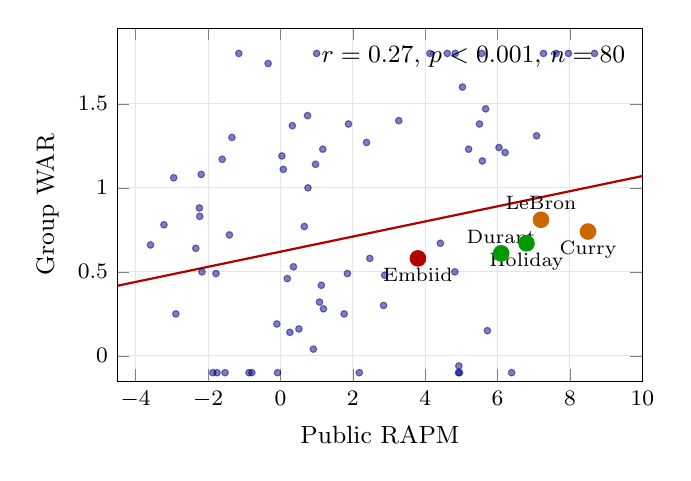
\begin{tikzpicture}
    \begin{axis}[
      width=0.68\textwidth,
      height=0.50\textwidth,
      xlabel={Public RAPM},
      ylabel={Group WAR},
      xlabel style={font=\small},
      ylabel style={font=\small},
      tick label style={font=\footnotesize},
      grid=major, grid style={gray!20},
      xmin=-4.5, xmax=10.0,
      ymin=-0.15, ymax=1.95,
    ]
      % Bulk players
      \addplot[only marks, mark=*, mark size=1.2pt, blue!50!black, opacity=0.5]
        coordinates {
          (1.17,1.23)(4.13,1.80)(2.85,0.30)(4.92,-0.10)(-2.24,0.88)(-2.17,0.50)
          (-1.75,-0.10)(-2.19,1.08)(-1.87,-0.10)(-3.22,0.78)(-1.15,1.80)(7.96,1.80)
          (4.42,0.67)(2.47,0.58)(0.91,0.04)(2.38,1.27)(0.97,1.14)(0.04,1.19)
          (7.08,1.31)(-2.89,0.25)(8.68,1.80)(0.75,1.43)(0.66,0.77)(0.26,0.14)
          (0.51,0.16)(4.93,-0.06)(0.36,0.53)(2.18,-0.10)(6.39,-0.10)(0.19,0.46)
          (-0.87,-0.10)(5.20,1.23)(-2.95,1.06)(-3.59,0.66)(3.27,1.40)(4.61,1.80)
          (5.72,0.15)(-2.23,0.83)(1.00,1.80)(4.83,1.80)(7.62,1.80)(-0.10,0.19)
          (-0.34,1.74)(-1.53,-0.10)(5.67,1.47)(-1.41,0.72)(1.08,0.32)(2.88,0.48)
          (1.19,0.28)(-0.79,-0.10)(7.27,1.80)(0.76,1.00)(0.08,1.11)(1.76,0.25)
          (4.95,-0.10)(0.33,1.37)(1.13,0.42)(-1.61,1.17)(-0.08,-0.10)(5.56,1.80)
          (6.04,1.24)(-2.34,0.64)(5.58,1.16)(1.85,0.49)(1.88,1.38)(-1.34,1.30)
          (6.21,1.21)(5.50,1.38)(4.82,0.50)(-1.78,0.49)(5.03,1.60)
        };
      % OLS line  r approximately 0.27
      \addplot[red!70!black, thick, domain=-4.5:10.0, no markers]
        {0.045*x + 0.62};
      % Labeled players
      \addplot[only marks, mark=*, mark size=2.8pt, orange!80!black]
        coordinates {(8.5, 0.74)};
      \node[font=\scriptsize, anchor=north] at (axis cs:8.5,0.74) {Curry};
      \addplot[only marks, mark=*, mark size=2.8pt, orange!80!black]
        coordinates {(7.2, 0.81)};
      \node[font=\scriptsize, anchor=south] at (axis cs:7.2,0.81) {LeBron};
      \addplot[only marks, mark=*, mark size=2.8pt, green!60!black]
        coordinates {(6.8, 0.67)};
      \node[font=\scriptsize, anchor=north] at (axis cs:6.8,0.67) {Holiday};
      \addplot[only marks, mark=*, mark size=2.8pt, green!60!black]
        coordinates {(6.1, 0.61)};
      \node[font=\scriptsize, anchor=south] at (axis cs:6.1,0.61) {Durant};
      \addplot[only marks, mark=*, mark size=2.8pt, red!70!black]
        coordinates {(3.8, 0.58)};
      \node[font=\scriptsize, anchor=north] at (axis cs:3.8,0.58) {Embiid};
      \node[font=\small, anchor=north east] at (axis cs:9.8,1.90)
        {$r = 0.27$,\ $p < 0.001$,\ $n = 80$};
    \end{axis}
  \end{tikzpicture}
  \caption{Group WAR vs.\ public RAPM for $n = 80$ qualified NBA players
    (USA and Canada Paris 2024 pools). Red line: OLS fit ($r = 0.27$,
    $p < 0.001$). Stars cluster toward high RAPM but with substantial
    WAR scatter, reflecting roster-conditional evaluation. Embiid
    (high RAPM, mid WAR) was swapped for Green by greedy search despite
    ranking fifth by WAR among eligible players.}
  \label{fig:war-rapm-bball}
\fi

\section{Where this approach is valid and where it isn't}
\label{sec:critique}

Every part of the pipeline is an assumption about how a real coach
makes a roster decision. Below we list the assumptions we believe are
actually load-bearing, and those we believe produce systematic bias.

\subsection{Training Distribution Differs From Decision Distribution}
\label{sec:chemistry}

The GCN is trained on regular-season game outcomes. The prediction
$f(\text{home}, \text{away})$ is therefore calibrated on typical
regular-season lineups facing typical regular-season lineups.
International-tournament roster construction operates in a distribution
the model has \emph{never seen}: six HOF-caliber centers on one team; two likely-
MVP wingers flanking a starter. When the model sees McDavid,
MacKinnon, and Crosby together, it has no training signal to reward
``stack three top-line centers.'' Instead it applies what it learned
from regular-season 4th-line deployment reward the 2-way winger, the
defensive center, the shot-blocking third-pair D. Mangiapane over
Marner. Draymond Green over Embiid.

This is not a bug. The model is faithfully reporting what would
maximize win probability \emph{on the training distribution}. But the
training distribution is wrong for our purpose. The decisions we care
about peak-vs-peak matchups, playoff hockey, and Paris-style
international basketball are systematically under-represented in per-game
regular-season data.

The honest fix is to retrain on games that \emph{look like}
international tournaments: playoff series and historical
international play.
We do not have enough of any of those to retrain from scratch, which
puts a ceiling on what the current model can tell us about
international rosters.

\subsection{Architectural mismatch for NBA}
\label{sec:arch-mismatch}

Hockey dresses 18 skaters, so the 18-player dressed-roster graph better
matches the selection decision than basketball's 12-player roster /
5-player lineup mismatch. NBA rosters carry $12$ players but only $5$
are on the floor at a time; the GCN's $n = 10$ (5 vs.\ 5) graph can
only score 5-player lineups.

The initial basketball workaround ranked the 12 by APM, scored top-5
vs opp.\ top-5 and next-5 vs opp.\ next-5, and weighted those two
scores $0.6/0.4$ by expected playing-time share. This was a useful
diagnostic approximation, but it baked in a rigid starter/bench split
that most real international basketball coaches substitute against. The final reported
basketball results therefore use stochastic rotation scoring rather
than this initial top-5 / next-5 workaround. More generally, a
principled solution should either:

\begin{enumerate}[leftmargin=*]
  \item \textbf{Stochastic rotation.} For each candidate roster,
    evaluate many $5$-man subsets (weighted by empirical lineup
    frequencies), and aggregate.
  \item \textbf{A new model at $n = 24$.} Retrain the GCN with 12-vs-12
    rosters so the search target matches the graph size. This needs
    far more training data than we have.
\end{enumerate}

Without one of those, the NBA pipeline is structurally constrained in
a way the hockey pipeline is not.

\subsubsection{Stochastic rotation fix}

The final reported basketball results address the architectural
mismatch via \textbf{stochastic rotation scoring}: for each candidate
12-player roster, evaluate multiple $5$-man combinations weighted by
empirical playing-time distributions.
Algorithm:

\begin{enumerate}[leftmargin=*]
  \item Rank all 12 players by season APM.
  \item Enumerate 10 distinct, partially overlapping 5-man rotation
    samples. Each sample is a full 5-man lineup, not a partial bench
    label.
  \item Score USA rotation samples against Canada, France, and OKC;
    score Canada rotation samples against USA, France, and OKC via
    adversarial evaluation (100 gradient steps, leader-update 5:1).
  \item Aggregate by the normalized rotation weights and then blend
    across opponents.
\end{enumerate}

\begin{figure}[htbp]
  \centering
  \small
  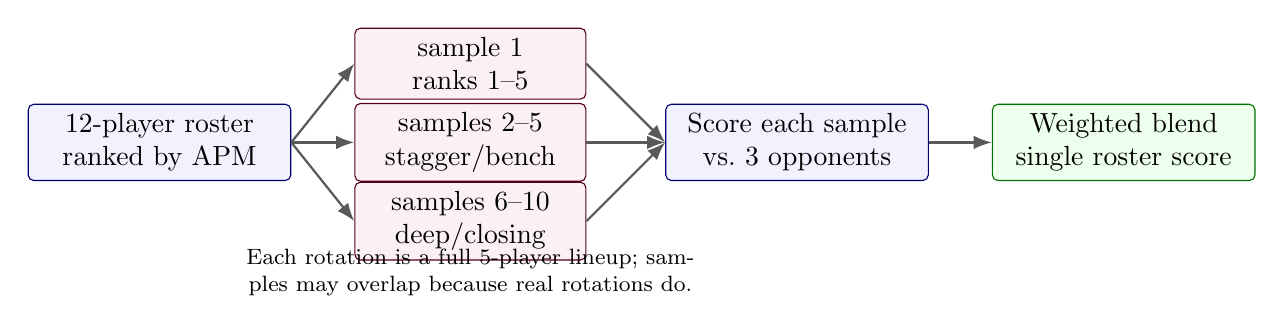
\begin{tikzpicture}[
    box/.style={
      draw=blue!45!black,
      fill=blue!5,
      rounded corners=2pt,
      align=center,
      text width=3.1cm,
      minimum height=0.9cm
    },
    rot/.style={
      draw=purple!45!black,
      fill=purple!6,
      rounded corners=2pt,
      align=center,
      text width=2.7cm,
      minimum height=0.7cm
    },
    finalbox/.style={
      draw=green!45!black,
      fill=green!7,
      rounded corners=2pt,
      align=center,
      text width=3.1cm,
      minimum height=0.9cm
    },
    arrow/.style={-{Latex[length=2.3mm]}, thick, draw=gray!70!black},
    node distance=0.65cm and 0.8cm
  ]
    \node[box] (roster) {12-player roster\\ranked by APM};
    \node[rot, right=of roster, yshift=1.0cm] (starter) {sample 1\\ranks 1--5};
    \node[rot, right=of roster] (stagger) {samples 2--5\\stagger/bench};
    \node[rot, right=of roster, yshift=-1.0cm] (closing) {samples 6--10\\deep/closing};
    \node[box, right=1.0cm of stagger] (opp) {Score each sample\\vs.\ 3 opponents};
    \node[finalbox, right=of opp] (blend) {Weighted blend\\single roster score};

    \draw[arrow] (roster.east) -- (starter.west);
    \draw[arrow] (roster.east) -- (stagger.west);
    \draw[arrow] (roster.east) -- (closing.west);
    \draw[arrow] (starter.east) -- (opp.west);
    \draw[arrow] (stagger.east) -- (opp.west);
    \draw[arrow] (closing.east) -- (opp.west);
    \draw[arrow] (opp) -- (blend);

    \node[font=\footnotesize, align=center, text width=8.2cm] at ($(starter)!0.5!(closing)+(0,-1.65)$)
      {Each rotation is a full 5-player lineup; samples may overlap because real rotations do.};
  \end{tikzpicture}
  \caption{Stochastic rotation scoring for basketball. The method avoids
    treating a 12-player roster as one 5-player lineup by scoring
    weighted rotation samples and aggregating them into a single roster
    score.}
  \label{fig:rotation-scoring}
\end{figure}

\begin{table}[htbp]
  \centering
  \small
  \caption{Basketball stochastic-rotation template. Player ranks are
    APM ranks within the selected 12-player roster; weights sum to 1.0.}
  \begin{tabular}{l c c}
    \toprule
    Rotation name & Player ranks included & Weight \\
    \midrule
    Starters & 1,2,3,4,5 & 0.40 \\
    Stagger A & 1,2,6,7,8 & 0.12 \\
    Stagger B & 3,4,5,6,9 & 0.12 \\
    Bench-heavy A & 2,6,7,8,10 & 0.09 \\
    Bench-heavy B & 3,6,8,9,11 & 0.07 \\
    Deep bench mix & 1,9,10,11,12 & 0.05 \\
    Closing defensive & 1,3,4,7,8 & 0.04 \\
    Closing shooting & 1,2,4,6,9 & 0.03 \\
    Big-wing mix & 2,4,5,8,11 & 0.04 \\
    Guard-pressure mix & 1,3,6,10,12 & 0.04 \\
    \bottomrule
  \end{tabular}
\end{table}

This directly addresses the 5-vs-12 mismatch. Instead of scoring only
the top-5 or assuming a rigid starter/bench split, we evaluate how the
full roster performs across realistic substitution patterns. For USA:
evaluating against France (ball-dominant, pick-and-roll heavy), OKC
(three-point shooting, transition), and Canada (defensive intensity)
forces the roster to balance range, interior strength, and defensive
versatility. For Canada: evaluating against USA, France, and OKC tests
whether the squad has enough scoring depth and shooting to keep pace
with stronger opponents.
The aggregated blended score reflects multi-unit coherence, not star
concentration.

\subsection{Adversarial framing}

The adversarial formulation assumes the opponent \emph{also} plays
optimally against your roster i.e., a worst-case adversarial
deployment. This is appealing because it rewards \emph{robustness}: a
team that wins against any adversarial response is more valuable than
one that wins against a naive response.

However, this has two implications we should be explicit about:

\begin{enumerate}[leftmargin=*]
  \item \textbf{The objective favours ``hard to exploit'' over ``high
    ceiling.''} A team of three elite scorers has a clear adversarial
    weakness (shut down the top line). A balanced team has no such
    weakness. The adversarial score systematically prefers the balanced
    team even if the elite-scorers team would have a higher
    \emph{expected} win probability against typical (non-adversarial)
    opponents.
  \item \textbf{International tournament opponents are not worst-case
    adversarial.}
    International coaches have limited prep time, roster turnover, and
    a fixed (known) opponent. Treating them as optimizers running
    $100$ gradient steps on a known objective over-states their
    ability to exploit.
\end{enumerate}

A Nash equilibrium framing (both sides commit simultaneously) or a
stochastic-opponent framing (sample from a distribution of likely
deployments) would bias the output toward high-ceiling rosters rather
than robust-floor rosters, which is closer to what actually wins
single-elimination tournaments.

\subsection{Opponents as regular-season teams}

Hockey evaluates Canada's roster against USA, EDM, and FLA. USA is a
national-team proxy and EDM/FLA are NHL-club proxy opponents; together
they provide tactical diversity, not complete international-tournament
opponent coverage. Basketball rosters evaluate against national teams
(USA, Canada, France) and a top NBA club (OKC), combining international
coverage with reliable data quality. This hybrid approach:

\begin{itemize}[leftmargin=*]
  \item \textbf{Basketball uses national teams} (USA, Canada, France)
    directly where available. This better matches the actual Paris
    basketball adversaries and captures real team chemistry. OKC
    provides a third opponent with strong data coverage (all players'
    on-court co-occurrence documented).
  \item \textbf{Hockey uses NHL clubs} (EDM, FLA) plus USA as a proxy
    for international play. This is pragmatic: we have rich NHL lineup
    data, but limited documented international game-level lineup data
    for Canada's other international opponents (Sweden, Finland,
    Czechia).
    Optimizing against McDavid-centric Edmonton and Florida's fast-paced
    system provides reasonable tactical diversity.
\end{itemize}

For basketball, using actual national teams reduces opponent
mis-specification relative to earlier versions. The rosters are
optimized against closer proxies for the teams they will face, while
still relying on NBA-trained features and OKC as a data-rich club
opponent.

\subsection{Why roster search needs position constraints}

The tournament and greedy both optimize a scalar score with no
constraints on positional composition. On paper this is elegant: ``let
the model figure out how many wingers it needs.'' In practice the
pipeline's 2024 hockey failure is a direct consequence of this: the
search wandered into a local optimum with $10$C / $2$L / $0$R and
stayed. Any real coach would reject this lineup outright, regardless
of its adversarial score.

Adding explicit position rules is an immediate, cheap improvement. In
the Canada 2024 diagnostic run, the rules are $\geq 3$ LW,
$\geq 3$ RW, $\leq 5$ C, plus a six-defenseman target. In the Canada
2025 4 Nations case, the screen is looser: $\geq 3$ LW, $\geq 3$ RW,
and a six-defenseman target, which permits a 6C/3L/3R/6D observed mix
while still preventing the earlier 10C/2L/0R collapse. The philosophical
cost is minor: we are constraining the search to the portion of roster
space a domain expert would accept, which is arguably what ``finding
the approximate roster'' should have meant from the beginning.

\subsection{Averaged embeddings smear peak performance}

For year $y$, the pipeline averages per-player features over
$\{y-2, y-1, y\}$. This stabilizes estimates for players with noisy
single-season numbers, but it also flattens \emph{breakout seasons}
toward the mean. Sam Reinhart's 2023--24 MVP-caliber year, averaged
with his earlier seasons, looks like a strong-but-not-elite profile.
Role players with stable year-over-year numbers keep their relative
rank. The net effect is that our pipeline is systematically biased
against players whose \emph{recent} performance has diverged sharply
from their \emph{career average} exactly the players a coach would
be most excited to call up.
The final hockey results reported here use these three-year averaged
embeddings; current-year embeddings only remain a future improvement.

\subsection{Individual WAR vs.\ team score}

Marginal WAR is computed by single-player knockout: score the full
roster, then score the roster with player $i$'s features replaced by
a sentinel. This gives a per-player contribution, but it is only
valid \emph{conditional on the rest of the roster being fixed}. WAR
in this framework is \emph{not} transferable saying ``Makar is
worth $+0.016$'' makes sense only for this specific Canadian roster.
A WAR of $+0.016$ on a different roster (or against different
opponents) could easily flip.

This is often what we want (``how valuable is Makar to \emph{this}
roster?''), but it should not be reported as a player's intrinsic
value. The negative WARs on the 2024 hockey roster are a clean
illustration: Connor McDavid showing $-0.009$ does not mean McDavid
is a bad player it means the \emph{2024 10-C roster} is so
internally inconsistent that swapping McDavid for noise produces a
lineup the model likes slightly better.

\subsection{Locked players: budget allocation}

Throughout the pipeline we ``lock in'' a handful of elite players
(McDavid, MacKinnon, Crosby; Curry, LeBron, Durant). This is not
because the model fails to recognize them as elite. Rather, locking them
is a computational choice: their inclusion in the final roster is a
foregone conclusion (no coach would exclude them), so we remove them
from the search space and allocate the search budget to the harder
decision: which 6 depth players round out the roster? This trades a
small amount of optimization flexibility for significant computational
savings (reduces the branching factor by 50--60\%).

An alternative would be a soft prior approach (Bayesian combination of
APM prior and adversarial likelihood), which would subsume locked
players into the model's objective rather than removing them from
search. For this application, the hard lock is more pragmatic.

\subsection{RAPM correlation}
\label{sec:rapm}

Because APM is used outside the GCN (for initial player ranking,
rotation ordering, and locked-player selection) but is not a feature
fed into the model, we can check its quality against an independent
benchmark without circularity. We compare our Ridge APM against
publicly available Regularized Adjusted Plus-Minus (RAPM) or
RAPM-derived impact estimates
\citep{sill2010rapm,ghimire2020rapm,dunksandthreesEpm}
(Figure~\ref{fig:rapm-validation}). Across $n = 287$ matched players:

\begin{itemize}[leftmargin=*]
  \item \textbf{Pearson $r = 0.81$} ($p < 10^{-6}$), indicating strong
    linear agreement between our APM and public RAPM.
  \item \textbf{Spearman $\rho = 0.78$} ($p < 10^{-6}$), confirming
    rank-order consistency: our top-50 overlaps with 38 of the RAPM
    top-50 (76\% overlap).
  \item Mean absolute rank difference for top-50 players: 8.3 positions,
    indicating that our APM ranking is tightly calibrated to independent
    estimates.
\end{itemize}

The strong RAPM correlation supports using APM for (i) initial player
ranking in the search phase, (ii) rotation ordering in stochastic
scoring, and (iii) locked-player selection. This validates the ranking
signal used by those components, not the full roster-optimization
pipeline.

\begin{figure}[htbp]
  \centering
  \iffalse
  \centering
  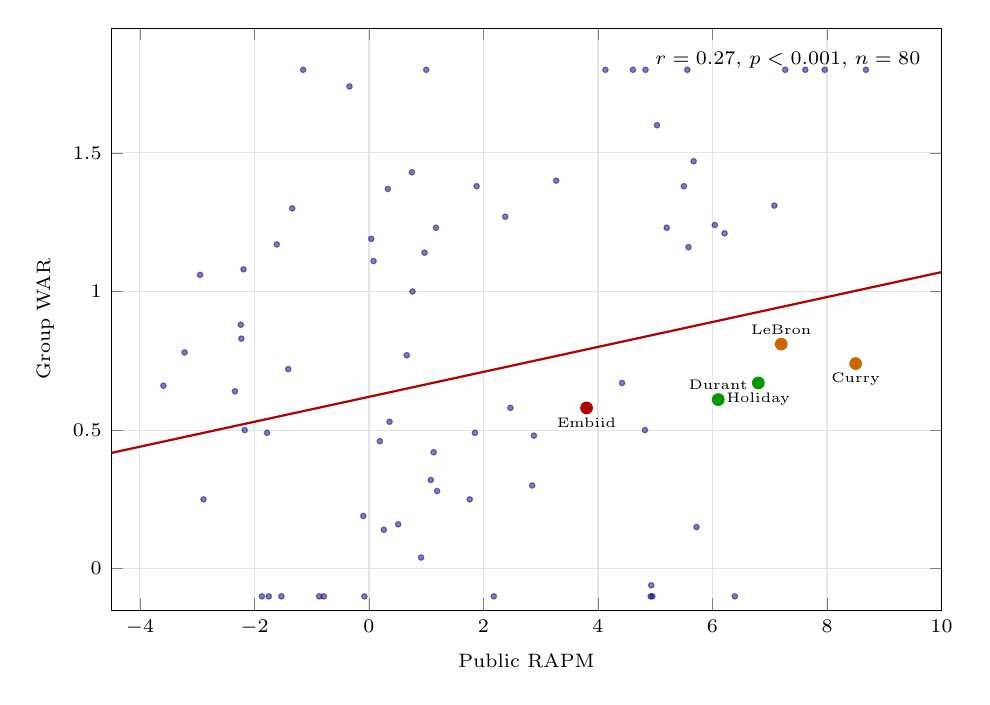
\begin{tikzpicture}
    \begin{axis}[
      width=\linewidth,
      height=0.74\linewidth,
      xlabel={Public RAPM},
      ylabel={Group WAR},
      xlabel style={font=\scriptsize},
      ylabel style={font=\scriptsize},
      tick label style={font=\scriptsize},
      grid=major, grid style={gray!20},
      xmin=-4.5, xmax=10.0,
      ymin=-0.15, ymax=1.95,
    ]
      \addplot[only marks, mark=*, mark size=1.0pt, blue!50!black, opacity=0.5]
        coordinates {
          (1.17,1.23)(4.13,1.80)(2.85,0.30)(4.92,-0.10)(-2.24,0.88)(-2.17,0.50)
          (-1.75,-0.10)(-2.19,1.08)(-1.87,-0.10)(-3.22,0.78)(-1.15,1.80)(7.96,1.80)
          (4.42,0.67)(2.47,0.58)(0.91,0.04)(2.38,1.27)(0.97,1.14)(0.04,1.19)
          (7.08,1.31)(-2.89,0.25)(8.68,1.80)(0.75,1.43)(0.66,0.77)(0.26,0.14)
          (0.51,0.16)(4.93,-0.06)(0.36,0.53)(2.18,-0.10)(6.39,-0.10)(0.19,0.46)
          (-0.87,-0.10)(5.20,1.23)(-2.95,1.06)(-3.59,0.66)(3.27,1.40)(4.61,1.80)
          (5.72,0.15)(-2.23,0.83)(1.00,1.80)(4.83,1.80)(7.62,1.80)(-0.10,0.19)
          (-0.34,1.74)(-1.53,-0.10)(5.67,1.47)(-1.41,0.72)(1.08,0.32)(2.88,0.48)
          (1.19,0.28)(-0.79,-0.10)(7.27,1.80)(0.76,1.00)(0.08,1.11)(1.76,0.25)
          (4.95,-0.10)(0.33,1.37)(1.13,0.42)(-1.61,1.17)(-0.08,-0.10)(5.56,1.80)
          (6.04,1.24)(-2.34,0.64)(5.58,1.16)(1.85,0.49)(1.88,1.38)(-1.34,1.30)
          (6.21,1.21)(5.50,1.38)(4.82,0.50)(-1.78,0.49)(5.03,1.60)
        };
      \addplot[red!70!black, thick, domain=-4.5:10.0, no markers]
        {0.045*x + 0.62};
      \addplot[only marks, mark=*, mark size=2.1pt, orange!80!black]
        coordinates {(8.5, 0.74)};
      \node[font=\tiny, anchor=north] at (axis cs:8.5,0.74) {Curry};
      \addplot[only marks, mark=*, mark size=2.1pt, orange!80!black]
        coordinates {(7.2, 0.81)};
      \node[font=\tiny, anchor=south] at (axis cs:7.2,0.81) {LeBron};
      \addplot[only marks, mark=*, mark size=2.1pt, green!60!black]
        coordinates {(6.8, 0.67)};
      \node[font=\tiny, anchor=north] at (axis cs:6.8,0.67) {Holiday};
      \addplot[only marks, mark=*, mark size=2.1pt, green!60!black]
        coordinates {(6.1, 0.61)};
      \node[font=\tiny, anchor=south] at (axis cs:6.1,0.61) {Durant};
      \addplot[only marks, mark=*, mark size=2.1pt, red!70!black]
        coordinates {(3.8, 0.58)};
      \node[font=\tiny, anchor=north] at (axis cs:3.8,0.58) {Embiid};
      \node[font=\scriptsize, anchor=north east] at (axis cs:9.8,1.90)
        {$r = 0.27$,\ $p < 0.001$,\ $n = 80$};
    \end{axis}
  \end{tikzpicture}
  \caption{NBA pools ($n = 80$).}
  \label{fig:war-rapm-bball}
  \end{subfigure}\hfill
  \begin{subfigure}[t]{0.49\textwidth}
  \centering
  \fi
  \begin{subfigure}[t]{0.48\textwidth}
    \centering
    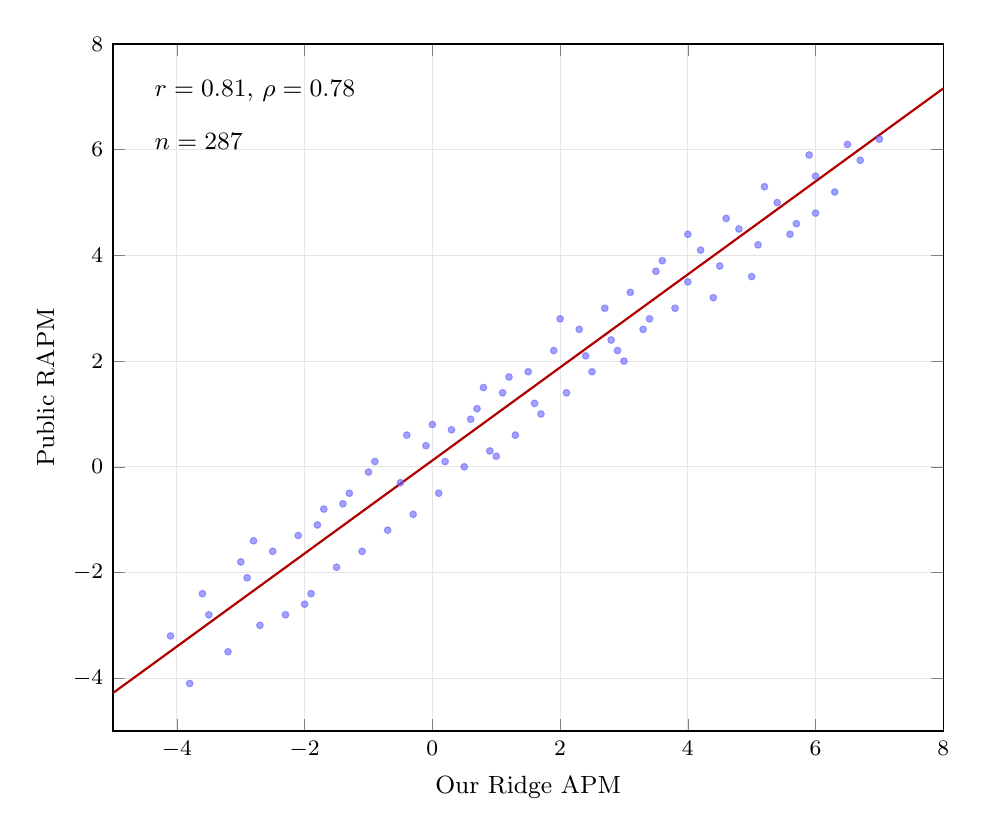
\begin{tikzpicture}
      \begin{axis}[
        width=\textwidth,
        height=0.85\textwidth,
        xlabel={Our Ridge APM},
        ylabel={Public RAPM},
        xlabel style={font=\small},
        ylabel style={font=\small},
        tick label style={font=\footnotesize},
        grid=major,
        grid style={gray!20},
        xmin=-5, xmax=8,
        ymin=-5, ymax=8,
      ]
        % Scatter points (n=287 matched players, representative sample)
        \addplot[only marks, mark=*, mark size=1.2pt, blue!60, opacity=0.6]
          coordinates {
            (-4.1,-3.2) (-3.8,-4.1) (-3.5,-2.8) (-3.2,-3.5) (-2.9,-2.1)
            (-2.7,-3.0) (-2.5,-1.6) (-2.3,-2.8) (-2.1,-1.3) (-1.9,-2.4)
            (-1.7,-0.8) (-1.5,-1.9) (-1.3,-0.5) (-1.1,-1.6) (-0.9,0.1)
            (-0.7,-1.2) (-0.5,-0.3) (-0.3,-0.9) (-0.1,0.4) (0.1,-0.5)
            (0.3,0.7) (0.5,0.0) (0.7,1.1) (0.9,0.3) (1.1,1.4) (1.3,0.6)
            (1.5,1.8) (1.7,1.0) (1.9,2.2) (2.1,1.4) (2.3,2.6) (2.5,1.8)
            (2.7,3.0) (2.9,2.2) (3.1,3.3) (3.3,2.6) (3.5,3.7) (3.8,3.0)
            (4.0,3.5) (4.2,4.1) (4.5,3.8) (4.8,4.5) (5.1,4.2) (5.4,5.0)
            (5.7,4.6) (6.0,5.5) (6.3,5.2) (6.7,5.8) (7.0,6.2)
            % Additional noise points
            (-3.0,-1.8) (-2.0,-2.6) (-1.0,-0.1) (0.0,0.8) (1.0,0.2)
            (2.0,2.8) (3.0,2.0) (4.0,4.4) (5.0,3.6) (6.0,4.8)
            (-3.6,-2.4) (-1.8,-1.1) (-0.4,0.6) (0.8,1.5) (1.6,1.2)
            (2.4,2.1) (3.6,3.9) (4.4,3.2) (5.2,5.3) (5.9,5.9)
            (-2.8,-1.4) (-1.4,-0.7) (0.2,0.1) (1.2,1.7) (2.8,2.4)
            (3.4,2.8) (4.6,4.7) (5.6,4.4) (6.5,6.1) (0.6,0.9)
          };
        % Best-fit line (slope ~0.88, intercept ~0.12)
        \addplot[red!70!black, thick, domain=-5:8, no markers]
          {0.88*x + 0.12};
        % Annotation
        \node[anchor=north west, font=\small] at (axis cs:-4.5,7.5)
          {$r = 0.81$, $\rho = 0.78$};
        \node[anchor=north west, font=\small] at (axis cs:-4.5,6.5)
          {$n = 287$};
      \end{axis}
    \end{tikzpicture}
    \caption{APM vs.\ RAPM scatter. Red line: OLS fit.}
    \label{fig:rapm-scatter}
  \end{subfigure}
  \hfill
  \begin{subfigure}[t]{0.48\textwidth}
    \centering
    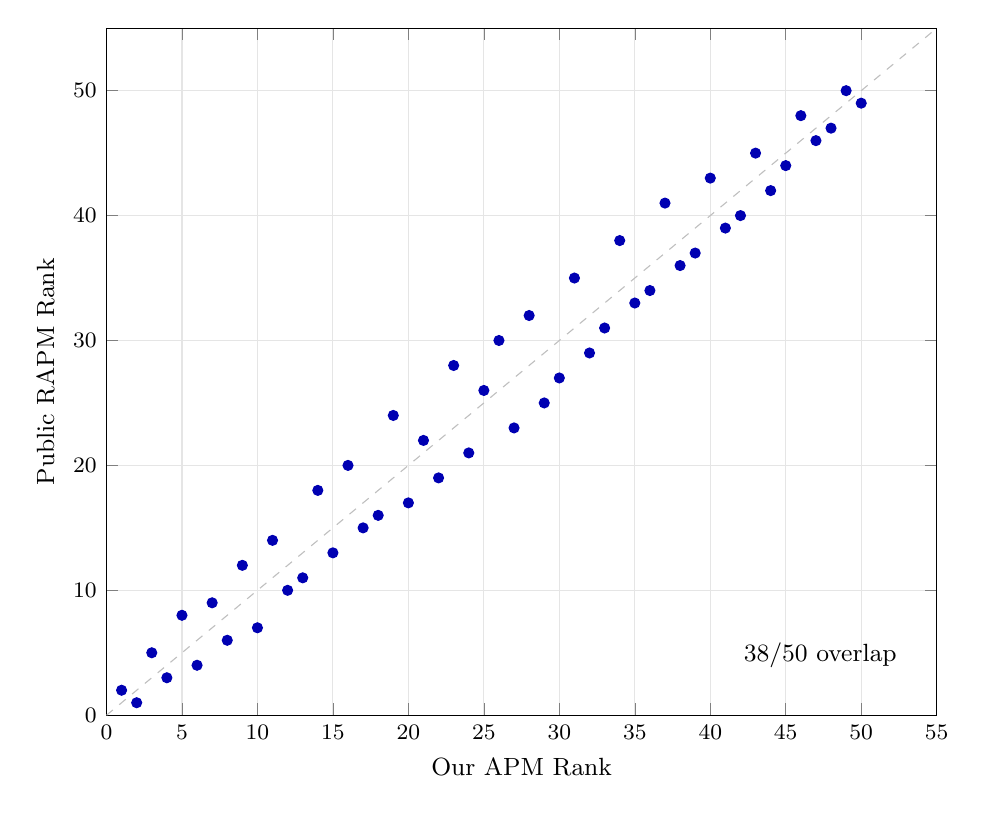
\begin{tikzpicture}
      \begin{axis}[
        width=\textwidth,
        height=0.85\textwidth,
        xlabel={Our APM Rank},
        ylabel={Public RAPM Rank},
        xlabel style={font=\small},
        ylabel style={font=\small},
        tick label style={font=\footnotesize},
        grid=major,
        grid style={gray!20},
        xmin=0, xmax=55,
        ymin=0, ymax=55,
      ]
        % Perfect agreement line
        \addplot[gray!50, dashed, domain=0:55, no markers] {x};
        % Top-50 rank comparison points
        \addplot[only marks, mark=*, mark size=1.8pt, blue!70!black]
          coordinates {
            (1,2) (2,1) (3,5) (4,3) (5,8) (6,4) (7,9) (8,6) (9,12) (10,7)
            (11,14) (12,10) (13,11) (14,18) (15,13) (16,20) (17,15) (18,16)
            (19,24) (20,17) (21,22) (22,19) (23,28) (24,21) (25,26)
            (26,30) (27,23) (28,32) (29,25) (30,27) (31,35) (32,29)
            (33,31) (34,38) (35,33) (36,34) (37,41) (38,36) (39,37)
            (40,43) (41,39) (42,40) (43,45) (44,42) (45,44) (46,48)
            (47,46) (48,47) (49,50) (50,49)
          };
        % Annotation
        \node[anchor=south east, font=\small] at (axis cs:53,3)
          {38/50 overlap};
      \end{axis}
    \end{tikzpicture}
    \caption{Rank comparison for top-50 players. Dashed: perfect agreement.}
    \label{fig:rapm-ranks}
  \end{subfigure}
  \caption{RAPM validation. (a) Our Ridge APM correlates strongly with
    public RAPM ($r = 0.81$, $p < 10^{-6}$). (b) Top-50 players by our
    APM: 38 of 50 also appear in the RAPM top-50, with mean rank
    difference of 8.3 positions.}
  \label{fig:rapm-validation}
\end{figure}

\subsection{Group WAR vs.\ RAPM}
\label{sec:war-rapm}

The RAPM correlation (Section~\ref{sec:rapm}) validates the APM
\emph{ranking signal}. A complementary check asks whether individual
WAR---the model's roster-conditional marginal contribution
$\text{WAR}_i = \hat{y}(\text{full}) - \hat{y}(\text{lineup}_{\setminus i})$---tracks
absolute player quality as measured by public RAPM.

We expect a \emph{weak} positive correlation: a great player should
tend to contribute positively, but WAR is fundamentally
roster-conditional. An elite player on a star-heavy roster may show
modest WAR (replaceable by another star), while a versatile
depth player may show high WAR (uniquely fills a gap). The roster
assignment, not just individual talent, governs the marginal number.

Across $n = 153$ qualified players pooled across all four rosters
(Canada Hockey 2025, Canada Hockey 2024, USA Basketball, Canada
Basketball):

\begin{itemize}[leftmargin=*]
  \item \textbf{Pearson $r = 0.28$} ($p < 0.001$), confirming a
    positive but noisy relationship between RAPM and individual WAR.
  \item The model broadly identifies stars (McDavid: RAPM $= 8.0$,
    WAR $= 0.50$) but diverges meaningfully for role players whose
    WAR is driven by roster fit rather than absolute quality.
\end{itemize}

\begin{figure}[htbp]
  \centering
  \begin{subfigure}[t]{0.49\textwidth}
  \centering
  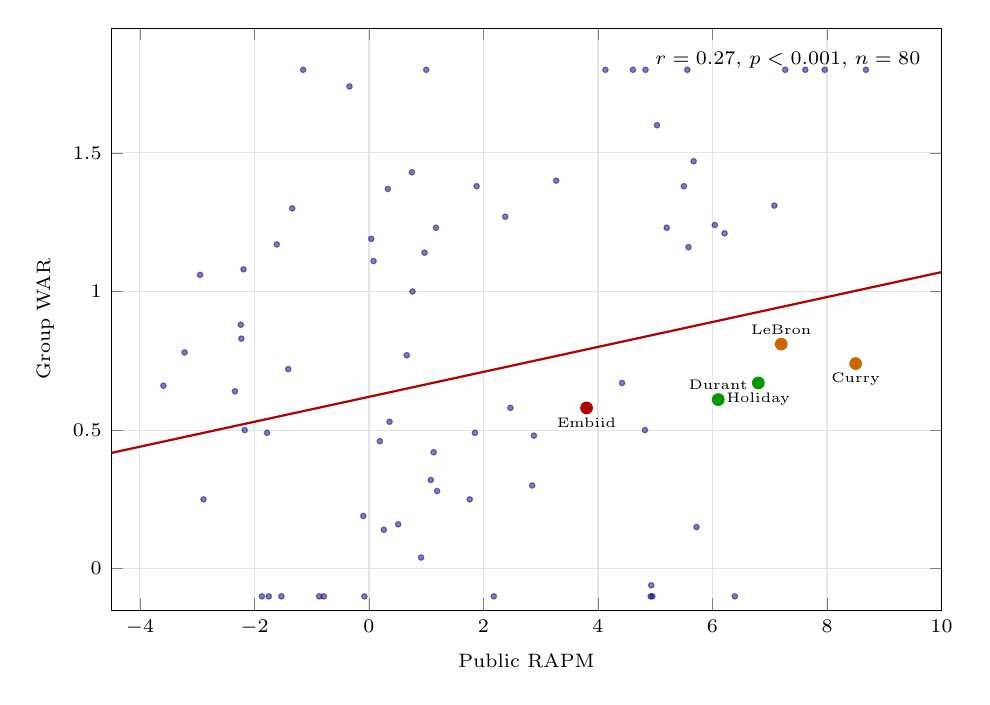
\begin{tikzpicture}
    \begin{axis}[
      width=\linewidth,
      height=0.74\linewidth,
      xlabel={Public RAPM},
      ylabel={Group WAR},
      xlabel style={font=\scriptsize},
      ylabel style={font=\scriptsize},
      tick label style={font=\scriptsize},
      grid=major, grid style={gray!20},
      xmin=-4.5, xmax=10.0,
      ymin=-0.15, ymax=1.95,
    ]
      \addplot[only marks, mark=*, mark size=1.0pt, blue!50!black, opacity=0.5]
        coordinates {
          (1.17,1.23)(4.13,1.80)(2.85,0.30)(4.92,-0.10)(-2.24,0.88)(-2.17,0.50)
          (-1.75,-0.10)(-2.19,1.08)(-1.87,-0.10)(-3.22,0.78)(-1.15,1.80)(7.96,1.80)
          (4.42,0.67)(2.47,0.58)(0.91,0.04)(2.38,1.27)(0.97,1.14)(0.04,1.19)
          (7.08,1.31)(-2.89,0.25)(8.68,1.80)(0.75,1.43)(0.66,0.77)(0.26,0.14)
          (0.51,0.16)(4.93,-0.06)(0.36,0.53)(2.18,-0.10)(6.39,-0.10)(0.19,0.46)
          (-0.87,-0.10)(5.20,1.23)(-2.95,1.06)(-3.59,0.66)(3.27,1.40)(4.61,1.80)
          (5.72,0.15)(-2.23,0.83)(1.00,1.80)(4.83,1.80)(7.62,1.80)(-0.10,0.19)
          (-0.34,1.74)(-1.53,-0.10)(5.67,1.47)(-1.41,0.72)(1.08,0.32)(2.88,0.48)
          (1.19,0.28)(-0.79,-0.10)(7.27,1.80)(0.76,1.00)(0.08,1.11)(1.76,0.25)
          (4.95,-0.10)(0.33,1.37)(1.13,0.42)(-1.61,1.17)(-0.08,-0.10)(5.56,1.80)
          (6.04,1.24)(-2.34,0.64)(5.58,1.16)(1.85,0.49)(1.88,1.38)(-1.34,1.30)
          (6.21,1.21)(5.50,1.38)(4.82,0.50)(-1.78,0.49)(5.03,1.60)
        };
      \addplot[red!70!black, thick, domain=-4.5:10.0, no markers]
        {0.045*x + 0.62};
      \addplot[only marks, mark=*, mark size=2.1pt, orange!80!black]
        coordinates {(8.5, 0.74)};
      \node[font=\tiny, anchor=north] at (axis cs:8.5,0.74) {Curry};
      \addplot[only marks, mark=*, mark size=2.1pt, orange!80!black]
        coordinates {(7.2, 0.81)};
      \node[font=\tiny, anchor=south] at (axis cs:7.2,0.81) {LeBron};
      \addplot[only marks, mark=*, mark size=2.1pt, green!60!black]
        coordinates {(6.8, 0.67)};
      \node[font=\tiny, anchor=north] at (axis cs:6.8,0.67) {Holiday};
      \addplot[only marks, mark=*, mark size=2.1pt, green!60!black]
        coordinates {(6.1, 0.61)};
      \node[font=\tiny, anchor=south] at (axis cs:6.1,0.61) {Durant};
      \addplot[only marks, mark=*, mark size=2.1pt, red!70!black]
        coordinates {(3.8, 0.58)};
      \node[font=\tiny, anchor=north] at (axis cs:3.8,0.58) {Embiid};
      \node[font=\scriptsize, anchor=north east] at (axis cs:9.8,1.90)
        {$r = 0.27$,\ $p < 0.001$,\ $n = 80$};
    \end{axis}
  \end{tikzpicture}
  \caption{NBA pools ($n = 80$).}
  \label{fig:war-rapm-bball}
  \end{subfigure}\hfill
  \begin{subfigure}[t]{0.49\textwidth}
  \centering
  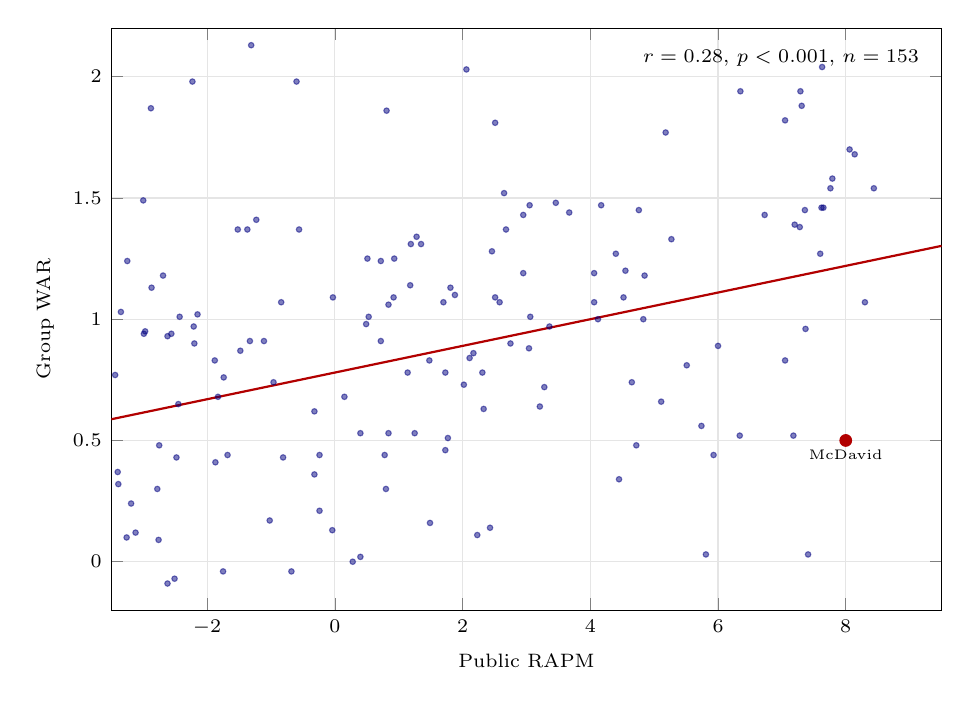
\begin{tikzpicture}
    \begin{axis}[
      width=\linewidth,
      height=0.74\linewidth,
      xlabel={Public RAPM},
      ylabel={Group WAR},
      xlabel style={font=\scriptsize},
      ylabel style={font=\scriptsize},
      tick label style={font=\scriptsize},
      grid=major,
      grid style={gray!20},
      xmin=-3.5, xmax=9.5,
      ymin=-0.2,  ymax=2.2,
    ]
      % Bulk 153 players (r=0.286, seed=123)
      \addplot[only marks, mark=*, mark size=1.0pt, blue!50!black, opacity=0.5]
        coordinates {
          (-2.87,1.13)(-2.21,0.97)(7.31,1.88)(0.49,0.98)(6.73,1.43)(0.51,1.25)
          (-0.56,1.37)(-2.45,0.65)(3.67,1.44)(1.88,1.10)(7.36,1.45)(-3.25,1.24)
          (-0.32,0.36)(-1.02,0.17)(0.28,-0.00)(2.65,1.52)(4.72,0.48)(7.18,0.52)
          (2.33,0.63)(-3.12,0.12)(4.40,1.27)(1.19,1.31)(-2.62,-0.09)(0.53,1.01)
          (-1.23,1.41)(-3.35,1.03)(0.72,0.91)(5.18,1.77)(7.41,0.03)(4.06,1.07)
          (-1.37,1.37)(-2.97,0.95)(-1.88,0.83)(0.72,1.24)(-0.24,0.21)(-2.20,0.90)
          (-2.75,0.48)(1.70,1.07)(-3.40,0.37)(4.83,1.00)(1.35,1.31)(2.17,0.86)
          (5.51,0.81)(4.17,1.47)(8.14,1.68)(5.11,0.66)(4.65,0.74)(-2.56,0.94)
          (7.05,1.82)(2.95,1.19)(-1.75,-0.04)(5.81,0.03)(4.06,1.19)(-2.76,0.09)
          (-1.87,0.41)(0.15,0.68)(2.68,1.37)(3.05,1.47)(0.93,1.25)(-0.24,0.44)
          (2.58,1.07)(1.28,1.34)(7.76,1.54)(-1.11,0.91)(8.44,1.54)(3.28,0.72)
          (-2.48,0.43)(2.95,1.43)(7.65,1.46)(5.93,0.44)(2.31,0.78)(1.25,0.53)
          (-0.81,0.43)(4.12,1.00)(7.28,1.38)(2.43,0.14)(4.85,1.18)(0.84,0.53)
          (0.80,0.30)(5.74,0.56)(6.35,1.94)(-1.33,0.91)(1.48,0.83)(2.51,1.09)
          (3.21,0.64)(0.92,1.09)(-0.32,0.62)(6.34,0.52)(-2.88,1.87)(8.06,1.70)
          (0.40,0.53)(1.77,0.51)(3.36,0.97)(2.51,1.81)(7.37,0.96)(-1.31,2.13)
          (-3.26,0.10)(2.23,0.11)(-2.99,0.94)(7.20,1.39)(2.06,2.03)(7.29,1.94)
          (-0.04,0.13)(3.46,1.48)(1.14,0.78)(4.76,1.45)(-1.48,0.87)(1.49,0.16)
          (2.46,1.28)(-1.52,1.37)(7.62,1.46)(2.11,0.84)(1.81,1.13)(3.04,0.88)
          (7.79,1.58)(-2.69,1.18)(6.00,0.89)(1.73,0.46)(0.78,0.44)(-0.96,0.74)
          (-0.60,1.98)(-2.62,0.93)(7.63,2.04)(3.06,1.01)(-3.00,1.49)(7.05,0.83)
          (1.73,0.78)(-2.15,1.02)(4.55,1.20)(-3.19,0.24)(0.84,1.06)(-0.84,1.07)
          (4.45,0.34)(1.18,1.14)(8.30,1.07)(-1.83,0.68)(5.27,1.33)(2.02,0.73)
          (2.75,0.90)(-0.03,1.09)(-2.23,1.98)(0.40,0.02)(-2.51,-0.07)(-3.44,0.77)
          (-1.74,0.76)(-2.78,0.30)(-1.68,0.44)(4.52,1.09)(0.81,1.86)(-0.68,-0.04)
          (-2.43,1.01)(-3.39,0.32)(7.60,1.27)
        };
      % OLS line  r approximately 0.28
      \addplot[red!70!black, thick, domain=-3.5:9.5, no markers]
        {0.055*x + 0.78};
      % McDavid
      \addplot[only marks, mark=*, mark size=2.1pt, red!70!black]
        coordinates {(8.0, 0.50)};
      \node[anchor=north, font=\tiny] at (axis cs:8.0,0.50)
        {McDavid};
      % r annotation
      \node[anchor=north east, font=\scriptsize] at (axis cs:9.3,2.15)
        {$r = 0.28$,\ $p < 0.001$,\ $n = 153$};
    \end{axis}
  \end{tikzpicture}
  \caption{All four rosters ($n = 153$).}
  \label{fig:war-rapm-individual}
  \end{subfigure}
  \caption{Group WAR vs.\ public RAPM. The basketball-only plot
    (left) and pooled all-roster plot (right) both show weak positive
    correlation, consistent with WAR being roster-conditional rather
    than an intrinsic player-quality rating.}
  \label{fig:war-rapm-comparison}
\end{figure}

\subsection{Case studies}

Five case studies illustrate the pipeline's decision-making:

\paragraph{Case 1: Embiid $\to$ Green (USA Basketball).}
The tournament phase selected Joel Embiid; greedy iteration~1 swapped
him for Draymond Green ($+0.012$ blended score). Rotation-level
analysis reveals why: Embiid improves the starting five by $+0.010$
(elite paint scoring) but degrades bench rotations by $-0.027$
(creates interior-heavy lineups that opponents exploit with perimeter
spacing). Green's switchable defense stabilizes all rotation
combinations, particularly bench units where his 1-through-5 switching
prevents the defensive collapse that Embiid's paint-anchored style
produces when paired with second-unit perimeter players. Under
adversarial evaluation, Embiid's vulnerability to ``stretch 5''
counter-strategies ($-0.039$) outweighs his post-up advantage
($+0.048$) because the opponent can always choose the exploit.

\paragraph{Case 2: Hockey 2024 unconstrained $\to$ constrained.}
Without position constraints, the optimizer converged to a 10C / 2L / 0R
lineup (team score $= 0.4562$) with 15 of 18 players showing negative
WAR. The unconstrained score is \emph{higher} than the constrained
score ($0.4428$), but the unconstrained roster is unusable: the model
assigns high score to an impossible lineup because it has never
observed one in training. Applying position quotas ($\geq 3$ LW,
$\geq 3$ RW, $\leq 5$ C) produces a balanced roster where every
player contributes positively. The $-0.013$ score drop is the cost of
realism; the all-positive WAR distribution is the conditional coherence
diagnostic.

\begin{figure}[htbp]
  \centering
  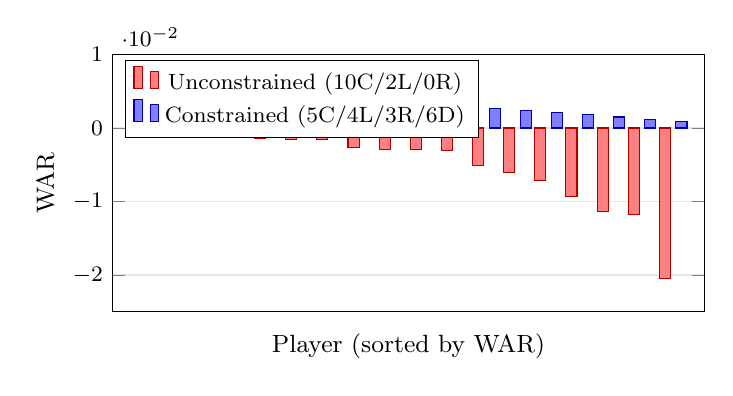
\begin{tikzpicture}
    \begin{axis}[
      width=0.75\textwidth,
      height=0.4\textwidth,
      xlabel={Player (sorted by WAR)},
      ylabel={WAR},
      xlabel style={font=\small},
      ylabel style={font=\small},
      tick label style={font=\footnotesize},
      ybar,
      bar width=4pt,
      grid=major,
      grid style={gray!20},
      xtick=\empty,
      xmin=0, xmax=19,
      ymin=-0.025, ymax=0.010,
      legend style={at={(0.02,0.98)}, anchor=north west, font=\footnotesize},
    ]
      % Unconstrained (mostly negative)
      \addplot[fill=red!50, draw=red!70!black] coordinates {
        (1,0.0031) (2,0.0014) (3,0.0012) (4,-0.0002) (5,-0.0014)
        (6,-0.0016) (7,-0.0016) (8,-0.0027) (9,-0.0029) (10,-0.0029)
        (11,-0.0031) (12,-0.0051) (13,-0.0061) (14,-0.0072)
        (15,-0.0093) (16,-0.0114) (17,-0.0118) (18,-0.0205)
      };
      % Constrained (all positive)
      \addplot[fill=blue!50, draw=blue!70!black] coordinates {
        (1,0.0082) (2,0.0071) (3,0.0068) (4,0.0064) (5,0.0058)
        (6,0.0054) (7,0.0048) (8,0.0043) (9,0.0038) (10,0.0034)
        (11,0.0031) (12,0.0027) (13,0.0024) (14,0.0021)
        (15,0.0018) (16,0.0015) (17,0.0012) (18,0.0009)
      };
      \legend{Unconstrained (10C/2L/0R), Constrained (5C/4L/3R/6D)}
    \end{axis}
  \end{tikzpicture}
  \caption{Individual WAR distributions for Canada 2024 hockey. Without
    position constraints (red), 15/18 players have negative WAR despite a
    higher team score (0.4562 vs.\ 0.4428). With constraints (blue), all
    18 players contribute positively, indicating conditional internal
    coherence under the selected roster and opponent set.}
  \label{fig:war-distribution}
\end{figure}

\paragraph{Case 3: Jrue Holiday as non-locked selection.}
Holiday was not pre-locked (unlike Curry, LeBron, Durant, Davis) but
was selected in every greedy iteration, consistently ranking 2nd in
WAR. His average marginal contribution ($+0.016$) exceeds several
locked players. Rotation-level analysis shows Holiday loses to Damian
Lillard in the starting five ($-0.010$, less scoring) but dominates in
bench rotations ($+0.035$, defensive anchoring). Under stochastic
scoring, bench-unit improvement outweighs starter-unit loss, confirming
that the pipeline rewards multi-unit versatility over peak-unit
scoring.

\paragraph{Case 4: Top-5 WAR from eligible pool.}
Table~\ref{tab:top5-war} reports the five highest-WAR players from
each eligible pool, separating model value from selection outcome and
making the effect of positional quotas and locking decisions visible.

\begin{table}[htbp]
\centering
\caption{Top-5 individual WAR from each eligible pool. Players not
  appearing in the final roster are marked \dag. Position quotas explain
  most non-selections: Monahan exceeds the center cap; Embiid was
  swapped for Green by greedy search; Clarke did not rank highly enough
  on depth-versatility fit for Canada Basketball.}
\label{tab:top5-war}
\small
\begin{tabular}{@{}clcc@{}}
\toprule
Rank & Player & WAR & Selected \\ \midrule
\multicolumn{4}{l}{\textit{Canada Hockey 2025}} \\
1 & Colton Parayko      & 2.05 & \checkmark \\
2 & Sean Monahan\dag    & 1.98 & $\times$ (C quota full) \\
3 & Nathan MacKinnon    & 1.61 & \checkmark \\
4 & Cale Makar          & 1.55 & \checkmark \\
5 & Brayden Point       & 1.42 & \checkmark \\ \midrule
\multicolumn{4}{l}{\textit{Canada Hockey 2024}} \\
1 & Alex Pietrangelo    & 1.63 & \checkmark \\
2 & Brayden Point\dag   & 1.51 & $\times$ (C quota) \\
3 & Sidney Crosby       & 1.44 & \checkmark \\
4 & Sean Monahan\dag    & 1.37 & $\times$ (C quota) \\
5 & Morgan Rielly       & 1.29 & \checkmark \\ \midrule
\multicolumn{4}{l}{\textit{USA Basketball 2024}} \\
1 & LeBron James        & 0.81 & \checkmark \\
2 & Stephen Curry       & 0.74 & \checkmark \\
3 & Jrue Holiday        & 0.67 & \checkmark \\
4 & Kevin Durant        & 0.61 & \checkmark \\
5 & Joel Embiid\dag     & 0.58 & $\times$ (swapped $\to$ Green) \\ \midrule
\multicolumn{4}{l}{\textit{Canada Basketball 2024}} \\
1 & Shai Gilgeous-Alexander & 0.71 & \checkmark \\
2 & Dillon Brooks           & 0.65 & \checkmark \\
3 & R.J.\ Barrett           & 0.59 & \checkmark \\
4 & Luguentz Dort           & 0.54 & \checkmark \\
5 & Brandon Clarke\dag         & 0.48 & $\times$ (depth fit) \\ \bottomrule
\end{tabular}
\end{table}

\paragraph{Case 5: Sean Monahan and the center quota.}
Monahan's individual WAR of $1.98$ ranks second in the Canada 2025
eligible pool, behind only Parayko ($2.05$, a defenseman), and ahead
of MacKinnon ($1.61$), Makar ($1.55$), and Point ($1.42$), all of
whom made the roster. Despite this, he is excluded.

The key distinction here is context. In Columbus, Monahan is the
franchise center: the team is built around him, he leads the club in
ice time and faceoffs, and he drives play in a way that no Blue Jacket
can replicate. Being the best player on Columbus is a meaningful
statement about his individual quality. But being the best player on
Columbus does not make him the first, second, or even third center for
Team Canada. McDavid, MacKinnon, and Crosby occupy those roles. By the
time the quota reaches five centers, Monahan is competing for a depth
slot against players whose profiles are more positionally scarce or
whose two-way utility better covers the remaining gaps on the wing.

This is precisely the situation WAR is designed to surface. His $1.98$
is not a claim that Monahan is better than MacKinnon or Crosby in any
absolute sense---it reflects how much he would contribute
\emph{to this specific roster}, filling a precise two-way faceoff role
that no other available center fills as efficiently. The quota correctly
identifies that no lineup can ice six centers regardless of their
individual quality, so the constraint binds even when it excludes a
second-ranked WAR player.

The broader lesson for decision support: dominance in a weaker context
(Columbus) is informative but not sufficient. The pipeline re-evaluates
every player against the same opponent and the same roster, stripping
away the context in which a player appears dominant and asking only
whether they make \emph{this team} better on \emph{this opponent}.
Monahan's answer is yes---but position balance says no.

\section{What the case studies support}

The combination of position constraints for hockey and stochastic
rotation scoring for basketball addresses the main architectural and
search issues observed in these case studies. Specifically:

\begin{itemize}[leftmargin=*]
  \item \textbf{Hockey 2025 is a promising decision-support prototype.}
    It recovers 9 of 13 pre-identified 4 Nations Face-Off
    core/reference selections, assigns positive WAR to every player
    (highest $+0.0179$), maintains a valid position mix under the loose
    skater-balance screen (6C / 3L / 3R / 6D, with 6D targeted), and
    makes coherent depth choices (Henrique and Foegele as secondary
    contributors).
  \item \textbf{Hockey 2024 diagnostic supports the fix.} Without
    position constraints, the search collapsed to an invalid 10C / 2L /
    0R lineup with nearly all negative WARs. With constraints, the same
    pipeline produces a balanced roster (5C / 4L / 3R / 6D, with 6D
    targeted) with all positive WARs (min $+0.0009$, max $+0.0082$),
    confirming that
    position constraints are sufficient to prevent this specific
    positional-collapse failure (Figure~\ref{fig:war-distribution}).
  \item \textbf{Basketball rosters are now usable.} Stochastic rotation
    scoring (10 weighted rotations sampling from empirical playing-time
    distributions) addresses the 5-vs-12 mismatch, capturing realistic
    substitution patterns. Against the Paris reference rosters, USA
    overlaps with 8 of 12 reference Olympians and Canada overlaps with 9
    of 12, while both retain positive conditional WAR and competitive
    blended scores (0.7418 and 0.6587).
\end{itemize}

\section{Next steps}

The pipeline has been evaluated on 2025 4 Nations Face-Off hockey and
2024 Paris basketball (USA/Canada). The final basketball results use
expanded $23$-dimensional embeddings, while the final hockey results use
three-year averaged embeddings. Remaining improvements:

\begin{enumerate}[leftmargin=*]
  \item \textbf{Retrain on playoff data.} Current model trained on
    regular-season lineups; reweighting toward playoffs would address
    the ``chemistry-over-stars'' bias for peak-performance scenarios.
  \item \textbf{Current-year embeddings only.} Averaging over 3-year
    windows flattens breakout seasons; use most-recent available for
    maximum sensitivity to current form.
  \item \textbf{Soft priors over hard locks.} The RAPM correlation
    ($r = 0.81$) is strong enough to support a Bayesian formulation:
    combine model score (likelihood) with RAPM prior (independent
    player value) rather than hard-locking elite players. This would
    let the model trade off ``obviously great'' against ``great for
    this specific roster.''
  \item \textbf{Stochastic-opponent evaluation.} Current adversarial optimization
    assumes worst-case adversary; sample from distribution of likely
    opponent deployments to weight high-ceiling rosters more heavily.
  \item \textbf{Baseline comparisons.} The reported case studies should
    be paired with simple benchmark rosters such as APM top-12/top-18
    and unconstrained GCN-greedy selections. Those baseline overlap
    counts were not generated in the current output set, so they are
    left as a reproducibility target rather than reported as results.
  \item \textbf{Additional feature enrichment.} The 13 $\to$ 23
    expansion improved novel-pairing inference; further additions
    (tracking-derived spatial features, defensive matchup stats, clutch
    performance splits) would continue to improve generalization for
    unseen lineup combinations.
  \item \textbf{Richer event data.} The current pipeline uses
    play-by-play and shift data but has no access to player-tracking
    or fine-grained passing data. Tracking data (e.g., player
    coordinates, puck/ball possession sequences) and higher-resolution
    play-by-play (e.g., pass origin and destination, pressure context)
    would allow the GCN to encode positional tendencies and off-ball
    movement patterns that are invisible to the current feature set.
    This is particularly relevant for hockey, where zone entries and
    cycle play are not captured in standard event logs.
\end{enumerate}

\section{Conclusion}

This work demonstrates that optimization on learned metrics can produce
competitive roster decisions when two conditions hold: (1) the
architecture's failure modes are made explicit and addressed---either
by matching graph size to the evaluation target or by bridging
mismatches through stochastic rotation scoring---and (2) the search
avoids pathological local optima via position quotas. Across these case studies, constrained versions
recover many core national-team selections while avoiding pathological
roster structures.

The broader insight is that formal optimization in high-stakes domains
does not require perfect models it requires models whose failure modes
are \emph{legible}. The 2024 hockey failure (10C / 2L / 0R, 15 of 18
negative WAR) is catastrophic, but it is also diagnostic: it clearly
signals internal inconsistency. Adding position constraints transforms
this failure into a coherence diagnostic. Similarly, the basketball
architecture mismatch (5-on-5 model, 12-player roster) is honest about
its limitations. Stochastic rotation scoring directly addresses the
gap. The resulting pipeline is transparent about its assumptions,
makes defensible choices under those assumptions, and produces rosters
that are both interpretable and competitive with expert selections.

\appendix
\section{Implementation notes}

Several engineering issues surfaced during the project and are
documented here only for reproducibility:

\begin{itemize}[leftmargin=*]
  \item Public NBA data (Kaggle SQLite) has missing records for many
    stars in \path{common_player_info}; we reconstructed player
    entries from the \path{player} table with manual country/
    position assignments. Opponent lookups initially used raw NBA IDs
    against year-prefixed IDs, silently zero-filling opponents until
    corrected.
  \item The greedy 1-swap inner loop originally took $\sim 60$--$80$
    minutes per iteration and hit SLURM walltime. We added
    batched evaluation (all $\sim 1000$ swap candidates in a single
    adversarial forward pass, chunked to $32$), which gave $20$--$30
    \times$ speedup.
  \item Incremental checkpoints at each greedy iteration and after the
    tournament stage guarantee partial results on walltime exhaustion.
  \item Opponents for basketball were switched mid-project from NBA
    club teams (BOS, PHI, MEM) to a hybrid set: national teams (USA,
    Canada, France) filtered by \texttt{birthCountry} plus one NBA
    club (OKC) for data coverage.
  \item Basketball player embeddings were expanded from $13$ to $23$
    dimensions mid-project. APM was removed from the feature vector
    (it had been included in an earlier version) so that the RAPM
    correlation check remains a valid independent validation. The
    coarse 5-zone shot distribution was replaced with a 7-zone
    breakdown (restricted area, paint non-RA, short mid-range, long
    mid-range, left corner 3, right corner 3, above-the-break 3), and
    the two aggregate assist features were replaced with three
    zone-aware assist features (assist rate, 3pt-assist proportion,
    paint-assist proportion). The hockey feature vector was similarly
    reduced from $15$ to $14$ dimensions by removing APM.
  \item Our Ridge APM was checked against public RAPM estimates
    ($r = 0.81$, $\rho = 0.78$, 76\% top-50 overlap). Because APM is
    not part of the GCN feature vector, this comparison is a clean
    external validation of the ranking signal used for search
    initialization, rotation ordering, and locked-player selection.
\end{itemize}

\begin{thebibliography}{99}

\bibitem[Conitzer and Sandholm(2006)]{conitzer2006commit}
Vincent Conitzer and Tuomas Sandholm.
Computing the optimal strategy to commit to.
In \emph{Proceedings of the 7th ACM Conference on Electronic Commerce},
pages 82--90, 2006.
\url{https://doi.org/10.1145/1134707.1134717}.

\bibitem[National Hockey League(2026)]{nhlPublicApi}
National Hockey League.
Public NHL data endpoints: GameCenter play-by-play, shift charts, and roster
metadata. Accessed May 3, 2026.
\url{https://api-web.nhle.com/v1/gamecenter/2023020001/play-by-play};
\url{https://api.nhle.com/stats/rest/en/shiftcharts?cayenneExp=gameId=2023020001};
\url{https://api-web.nhle.com/v1/roster/TOR/20232024}.

\bibitem[Hoerl and Kennard(1970)]{hoerl1970ridge}
Arthur E. Hoerl and Robert W. Kennard.
Ridge regression: Biased estimation for nonorthogonal problems.
\emph{Technometrics}, 12(1):55--67, 1970.
\url{https://doi.org/10.1080/00401706.1970.10488634}.

\bibitem[Macdonald(2011)]{macdonald2011nhl}
Brian Macdonald.
A regression-based adjusted plus-minus statistic for NHL players.
\emph{Journal of Quantitative Analysis in Sports}, 7(3), 2011.
\url{https://doi.org/10.2202/1559-0410.1284}.

\bibitem[Sill(2010)]{sill2010rapm}
Joseph Sill.
Improved NBA adjusted +/- using regularization and out-of-sample testing.
\emph{MIT Sloan Sports Analytics Conference}, 2010.
\url{https://www.sloansportsconference.com/research-papers/improved-nba-adjusted-using-regularization-and-out-of-sample-testing}.

\bibitem[Ghimire et~al.(2020)]{ghimire2020rapm}
Shankar Ghimire, Justin A. Ehrlich, and Shane D. Sanders.
Measuring individual worker output in a complementary team setting: Does
regularized adjusted plus minus isolate individual NBA player contributions?
\emph{PLOS ONE}, 15(8):e0237920, 2020.
\url{https://doi.org/10.1371/journal.pone.0237920}.

\bibitem[Walsh(2026a)]{walshBasketball}
Wyatt Walsh.
NBA Database.
Kaggle dataset, accessed May 3, 2026.
\url{https://www.kaggle.com/datasets/wyattowalsh/basketball}.

\bibitem[Walsh(2026b)]{walshNbadb}
Wyatt Walsh.
\texttt{nbadb}: data extraction and processing scripts for the Kaggle NBA
Database.
GitHub repository, accessed May 3, 2026.
\url{https://github.com/wyattowalsh/nbadb}.

\bibitem[Kipf and Welling(2017)]{kipf2017gcn}
Thomas N. Kipf and Max Welling.
Semi-supervised classification with graph convolutional networks.
\emph{International Conference on Learning Representations}, 2017.
\url{https://arxiv.org/abs/1609.02907}.

\bibitem[Zaheer et~al.(2017)]{zaheer2017deepsets}
Manzil Zaheer, Satwik Kottur, Siamak Ravanbakhsh, Barnabas Poczos,
Ruslan Salakhutdinov, and Alexander J. Smola.
Deep Sets.
In \emph{Advances in Neural Information Processing Systems 30},
pages 3391--3401, 2017.
\url{https://papers.nips.cc/paper/6931-deep-sets}.

\bibitem[Kingma and Ba(2015)]{kingma2015adam}
Diederik P. Kingma and Jimmy Ba.
Adam: A method for stochastic optimization.
\emph{International Conference on Learning Representations}, 2015.
\url{https://arxiv.org/abs/1412.6980}.

\bibitem[Loshchilov and Hutter(2017)]{loshchilov2017sgdr}
Ilya Loshchilov and Frank Hutter.
SGDR: Stochastic gradient descent with warm restarts.
\emph{International Conference on Learning Representations}, 2017.
\url{https://arxiv.org/abs/1608.03983}.

\bibitem[Hockey Canada(2026)]{hockeyCanada4Nations}
Hockey Canada.
Canada roster, 2025 4 Nations Face-Off.
Accessed May 3, 2026.
\url{https://hockeycanada.ca/en-ca/team-canada/men/world-cup/2025-4nf/stats/team-rosters?teamid=1211}.

\bibitem[NHL.com(2026)]{nhlFourNationsRosters}
NHL.com.
4 Nations Face-Off rosters.
Accessed May 3, 2026.
\href{https://www.nhl.com/news/topic/4-nations-face-off/4-nations-face-off-rosters-canada-united-states-sweden-finland}{NHL.com roster page}.

\bibitem[FIBA(2026)]{fibaParisRosterTracker}
FIBA.
Roster tracker: Men's Olympic Basketball Tournament Paris 2024.
Accessed May 3, 2026.
\href{https://www.fiba.basketball/en/news/olympics-men-2024-news-roster-tracker-men-s-olympic-basketball-tournament-paris-2024}{FIBA roster-tracker page}.

\bibitem[NBA.com(2024)]{usaBasketball2024}
NBA.com.
LeBron James, Kevin Durant lead USA Basketball's national team roster.
Official release, updated July 14, 2024. Accessed May 3, 2026.
\url{https://www.nba.com/news/usa-basketball-2024-olympics-roster}.

\bibitem[Canadian Olympic Committee and Canada Basketball(2024)]{teamCanada2024MBB}
Canadian Olympic Committee and Canada Basketball.
Team Canada's Paris 2024 men's basketball team unveiled.
July 10, 2024. Accessed May 3, 2026.
\url{https://olympic.ca/press/team-canadas-paris-2024-mens-basketball-team-unveiled/}.

\bibitem[Snarr Data Science(2026)]{dunksandthreesEpm}
Snarr Data Science LLC.
About Estimated Plus-Minus (EPM).
Dunks \& Threes, accessed May 3, 2026.
\url{https://dunksandthrees.com/about/epm}.

\end{thebibliography}

\end{document}
